
\chapter{Logaritmos e função logaritmica}
\section{Introdução}

Um dos grandes desafios da matemática no fim do século XVI e início do XVII era o desenvolvimento de meios para facilitar os cálculos aritméticos, evitando erros grosseiros e objetivando o auxílio a outras ciências. Nesse período em especial, as ciências que impulsionaram esses desenvolvimentos foram, a astronomia, que estava em alta na época e a navegação, influenciada pelo comércio mundial. Foram criados diversos métodos para facilitar os cálculos na época, porém a maioria deles fracassou por serem praticamente inviáveis ou de pouca precisão. Os logaritmos, na sua origem, foram criados como um meio de simplificar complexas operações de multiplicação e divisão, transformando-as em simples adições e subtrações.

John Napier (1550-1617) e Jobst Bürgi (1552-1632) são considerados pais da ideia de logaritmos conhecida hoje. Os trabalhos de Napier e Bürgi foram desenvolvidos independentes e quase que simultaneamente e tiveram focos diferentes no decorrer de seus trabalhos. Enquanto Napier desenvolveu seu trabalho a partir de noções geométricas, Bürgi trabalhou baseando-se em noções algébricas. 

É importante salientar também a importância de Michael Stifel (1487-1567), considerado um dos principais precursores dos logaritmos. Stifel publicou em 1544 o livro \textit{Arithmetica integra}, publicação de extrema importância para a álgebra da Alemanha no século XVI. É nessa obra que aparece uma origem para a ideia de logaritmo. Stifel descobre as vantagens de se fazer a associação entre uma progressão geométrica e uma progressão aritmética, um século antes da invenção dos logaritmos. Ele observou que o produto (quociente) de dois termos quaisquer da progressão geométrica está associado à soma (diferença) dos correspondentes na progressão aritmética.

Napier não era matemático profissional. Além de cuidar da administração de suas propriedades, se dedicou a escrever sobre vários assuntos. O termo logaritmo foi criado por ele e vem do latim, \textit{logos = }razão e \textit{arithmos =} número.\textit{ }Esse método, era para Napier, uma tentativa de expressar o cálculo a partir da razão ou da proporção numérica. Foi no ano de 1614, três anos antes de sua morte e seis anos antes da publicação de Bürgi, que John Napier publicou sua descoberta na obra intitulada de \textit{Mirifici logarithmorum canonis descriptio} (ou seja, \textit{Uma descrição da maravilhosa regra dos logaritmos}). Nesse livro, Napier explica através de sua concepção, os logaritmos, e junto disso fornece uma tábua dos logaritmos dos senos de 0º a 90º, de minuto em minuto. O motivo de Napier ter aplicado sua ideia à trigonometria foi devido ao fato que a intenção da criação dessa tabua de logaritmos era facilitar os extensos e complicados cálculos realizados pelos astrônomos e navegadores. Baseado nas publicações de Stifel, Napier deparou-se com a evidência de que as somas ou diferenças dos índices das potências eram na verdade produtos ou quocientes das potências dadas.

Observando a tabela a seguir é possível compreender a conclusão a qual Napier chegou: 

\begin{table}[H]
    \centering
    \begin{tabular}{lllllllllllllll}
    1 & 2 & 3 & 4  & \textbf{5}  & 6  & 7   & 8   & \textbf{9}   & 10   & 11   & 12   & 13   & \textbf{14} & 15    \\
    2 & 4 & 8 & 16 & \textbf{32} & 64 & 128 & 256 & \textbf{512} & 1024 & 2048 & 4096 & 8192 & 16384       & 32788
    \end{tabular}
\end{table}

Os números da primeira linha são os expoentes, enquanto a segunda linha contém as potências de 2 correspondentes a esses expoentes. Segundo a tabela, podemos calcular produtos complicados, como \textbf{32 x 512}, operando com uma simples operação de adição dos expoentes correspondentes. O expoente que corresponde ao 32 é o 5, e o expoente que corresponde ao 512 é o 9, dessa forma, o produto de 32 x 512 é igual a potência ~~~~~~~~~ 2\textsuperscript{5 + 9 }= 2\textsuperscript{14} = 16384.

Um ano após a publicação de seu livro, Napier foi a Edimburgo para encontrar Henry Briggs (1556-1630), matemático profissional de Londres. Durante o mês em que passaram juntos na cidade de Edimburgo, o assunto principal entre os dois, foi sem dúvidas os logaritmos. Após longas conversas, Napier e Briggs concluíram que uma tábua de logaritmos de base 10 seria mais útil, porém Napier não viveu o suficiente para o desenvolvimento dessa ideia. Briggs foi quem adaptou os valores de forma que fossem mais fáceis de serem utilizados por meio dos logaritmos decimais, como hoje os conhecemos.

Jobst Bürgi se dedicava à fabricação de relógios, mas tinha também talento para a matemática e para a astronomia, tendo realizado trabalhos em ambas as áreas. Assim como Napier, foi estimulado pelas ideias de Stifel, porém Bürgi partiu de uma progressão aritmética, com inicio no termo 0, com razão 10, e com último termo 32 000. A progressão geométrica correspondente inicia no 10\textsuperscript{8} e sua razão é 1 + 10\textsuperscript{-4}. A partir disso ele construiu uma tábua de antilogaritmos. Provavelmente Bürgi criou seus logaritmos por volta de 1600, mas só publicou uma obra sobre o assunto no ano de 1620, ficando assim atrás de Napier que publicou sua obra no de 1614.

Atualmente é possível encontrar diversas aplicações dos logaritmos na ciência e na engenharia. Seguem alguns exemplos: A definição do pH de uma solução química é na verdade um logaritmo, o logaritmo da quantidade de íons de H\textsuperscript{+}; a linearização de gráficos de funções exponenciais é feita~utilizando escala logarítmicas; o cálculo da meia-vida (tempo para decompor a metade da massa) de uma substância radioativa; o cálculo do tempo de permanência de uma substância no corpo humano é útil para determinar a  dosagem de medicamentos e usa logaritmos; o cálculo da depreciação de bens como carros e imóveis é feito usando funções exponenciais e logaritmos; a escala Richter, usada desde 1935, é uma escala logarítmica, por meio dela é possível calcular a magnitude (quantidade de energia liberada), epicentro e a amplitude de um terremoto; o crescimento ou decrescimento de populações é feito usando funções exponenciais e logaritmos, assim como o cálculo de aplicações financeiras como poupança, financiamentos e previdência.

\section{Definição de logaritmo}

Os logaritmos estão associados aos expoentes de potências. Analisemos os seguintes exemplos:

\begin{texemplo} 
    Que expoente \textit{N} deve ter \textit{2} , para que \textit{2\textsuperscript{N} = 8 } ? 

    \textbf{Solução:} Decompondo \textit{8} em fatores primos, temos\textit{: 8 = 2\textsuperscript{3}}. 

    \textit{2\textsuperscript{N} = 8 = 2\textsuperscript{3}}~~~~~~e~~~  \textit{N = 3}.

    Portanto, \textit{N = 3} é o expoente de \textit{2}, para que \textit{2\textsuperscript{N} = 8}\qedsymbol{}

\end{texemplo}

\begin{texemplo}
    Que expoente \textit{N} deve ter \textit{10,} para que \textit{10\textsuperscript{N} = 10000 } ? 

    \textbf{Solução:} Decompondo \textit{10000} em potencias de 10, temos: \textit{10000 = 10\textsuperscript{4}.} 

    \textit{10\textsuperscript{N} =~ 10\textsuperscript{4}~~~~~ }e~~~~ \textit{N = 4}.

    Portanto, \textit{N = 4} é o expoente de \textit{10}, para que \textit{10\textsuperscript{N} = 1000}\qedsymbol{}
\end{texemplo}

\begin{texemplo}
    Que expoente \textit{N} deve ter \textit{4,} para que \textit{4\textsuperscript{N} = 2 } ? 

    \textbf{Solução:} Decompondo \textit{4} em fatores primos, temos: \textit{4 = 2\textsuperscript{2}} 

    \(  \left( 2^{2} \right) ^{N} \) = 2~~~ 

    \( 2^{2N}=2^{1} \) ~~~ 

    \( 2N=1 \) ~~~~~~ e~~~~ \textit{N = 1/2.}

    Portanto, \textit{N = 1/2} é o expoente de \textit{4}, para que \textit{4\textsuperscript{N} = 2}\qedsymbol{}
\end{texemplo}

Chamando o expoente \textit{N} de $``$\textbf{logaritmo}$"$ , dizemos que determinar o logaritmo de um número \textit{x} em uma base \textit{b} é encontrar um expoente \textit{N} de \textit{b}, tal que \textit{b\textsuperscript{N} = x}.

No Ex. 2.1 o logaritmo de \textit{8} na base \textit{2} é \textit{N = 3}~ pois \textit{2\textsuperscript{3} = 8.}

No Ex. 2.2 o logaritmo de \textit{10000} na base \textit{10} é \textit{N = 4}~ pois \textit{10\textsuperscript{4} = 10000.}

No Ex. 2.3 o logaritmo de \textit{4} na base \textit{2} é \textit{N = 1/2}~ pois \textit{4\textsuperscript{1/2} = 2.}

\begin{caixa}
    \begin{tdefinicao}
        \( log_{b}x=N \Leftrightarrow b^{N}=x \) 
        \begin{flushright}
            (2.1)
        \end{flushright}

Onde \textit{N}, \textit{x} e \textit{b}~são~números~reais, sendo    \textit{x > 0};~ \textit{b > 0} e \textit{b $ \neq $  1}\qedsymbol{}

    \end{tdefinicao}
\end{caixa}

\begin{figure}[H]
	\begin{Center}
		\includegraphics[width=3.39in,height=2.44in]{capitulos/logaritmos_e_funcao_logaritmica/media/image2.png}
	\end{Center}
\end{figure}

~~

Na expressão~  \( log_{b}x=N \) , como indica a figura:

\textit{x} é o \textbf{logaritmando}, ou seja, o número que será calculado o logaritmo (também chamado de \textbf{antilogaritmo}),

\textit{b }é a \textbf{base} do logaritmo e

\textit{N }é o \textbf{logaritmo}\textit{.}

\begin{texemplo}
    Qual é o  \( log_{10}100 \)  ? ou qual deve ser o valor de \textit{N}~ para que \textit{10\textsuperscript{N} = 100} ?

    \textbf{Solução:} Utilizando a~definição do logaritmo, temos:  

    \[ log_{10}100=N \Leftrightarrow  10^{N}=100 \]

    \[ 10^{N}=10^{2} \] 

    \[ N=2 \]

Assim,dizemos que \( log_{10}100=2 \) pois \( 10^{2}=100 \) \qedsymbol{}
\end{texemplo}

\begin{texemplo}
    Qual é o logaritmo de \textit{81 }na base \textit{3} ?
    \textbf{Solução:} Usando a definição de logaritmo: \[ log_{3}81=N \Leftrightarrow 3^{N}=81 \] 

    Decompondo o \textit{81= 3\textsuperscript{4}}\textsuperscript{~~ }temos:~  \( 3^{N}=3^{4} \) ~~~~~ e~ \textit{N = 4}. 

    Dizemos~então que   \( log_{3}81=4  \)  pois  \textit{ 3\textsuperscript{4}}\textsuperscript{~ }\textit{= 81}\qedsymbol{}

\end{texemplo}

\begin{texemplo}
    Determine os valores de \textit{x} para que exista logaritmo \textit{N}:

    \begin{Center}
        \( log \left( 2x-1 \right)  \)  = \textit{N}
    \end{Center}

\textbf{Solução:} Da definição de logaritmo (2.1), o antilogaritmo deve ser maior do que zero. Então,

\textit{2x – 1 > 0} . Resolvendo para \textit{x}, temos:  \( x>\frac{1}{2} \) ~ .

Assim, para qualquer \textit{x > $\frac{1}{2}$} , o antilogaritmo será positivo e o logaritmo dado existirá.

\end{texemplo}

\begin{exercicios}
	\exitem{} Determine o valor do expoente \textit{N} para que as equações exponenciais sejam verdadeiras:

\begin{enumerate}
	\item \textit{5\textsuperscript{N} = 125\quad \quad }c) \textit{25\textsuperscript{N} = 125\quad \quad }e) \textit{9\textsuperscript{N} = 81}

	\item \textit{2\textsuperscript{N} = 64\quad }\quad d) \textit{5\textsuperscript{N} = 1/125\quad \quad }f)\textit{ 4\textsuperscript{N} = 1/32}
\end{enumerate}

	\exitem{} Calcule os seguintes logaritmos usando a definição:

\begin{enumerate}
	\item  \( log_{10}100000 \) \quad \quad d)  \( log_{5}125 \) \quad \quad g)  \( log_{2} \left( \frac{1}{32} \right)  \) 

	\item  \( log_{2} \left( \frac{1}{16} \right)  \) ~~~~ \quad \quad e)  \( log_{3}243 \) \quad \quad h)  \( log_{1/2}\sqrt[3]{4} \) 

	\item  \( log_{2}0,25 \) \quad \quad \quad f)  \( log_{81}3 \) \quad \quad i)  \( log_{0,01}10 \) 
\end{enumerate}

	\exitem{} Determine o valor da letra (use a definição de logaritmo). 

\begin{enumerate}
	\item  \( log_{9}x=2 \) \quad \quad c)  \( log_{b}5=125 \) \quad \quad e)  \( log_{7/6}36/49=N \) 

	\item  \( log_{b}8=3 \) \quad \quad d)  \( log_{ \left( x-2 \right) }8=2 \) \quad \quad f)  \( log_{6/7}36/49=x \) 
\end{enumerate}

	\exitem{} Verifique se tem sentido a base do logaritmo ser igual a 1. (Justifique sua resposta)

	\exitem{} Verifique se tem sentido a base do logaritmo ser um número negativo. (Justifique sua resposta)

	\exitem{} Verifique se tem sentido calcular o logaritmo de um número negativo. (Justifique sua resposta)

	\exitem{} Dê 5 exemplos de logaritmos negativos. Para que valores de \textit{x}, tem-se \(  log_{b}x \)  negativo?

	\exitem{} Determine os valores de \textit{x} para que exista logaritmo:

    \begin{enumerate}
	    \item  \( log \left( x-2 \right)  \) \quad b)  \( log_{3} \left( 4x-1 \right)  \) \quad c)  \( log_{ \left( 2x-1 \right) }5 \) \quad ~~~ d)  \( log_{ \left( 4-x \right) } \left( x-2 \right)  \) \quad 
    \end{enumerate}

\end{exercicios}

\section{Propriedades dos logaritmos}

As propriedades dos logaritmos são muito utilizadas para resolver problemas com equações e de aplicação de funções exponenciais. Todas elas decorrem diretamente ou são demonstradas usando a \textbf{Definição 2.1}.

\textbf{P1:~~ }\textit{log\textsubscript{b} 1 = 0}~~ \quad pois \textit{b\textsuperscript{0} = 1}.\quad \quad \quad \quad \quad \quad \quad (3.1)

\textbf{P2:}~~ \textit{log\textsubscript{b} b = 1}\quad pois~pela~Def. 2.1, tem-se:   ~ \textit{b\textsuperscript{1} = b}. \quad \quad \quad \quad \quad \quad \quad (3.2)

\textbf{P3:~~ }\textit{log\textsubscript{b} b\textsuperscript{n} = n}\quad pois pela Def. 2.1, tem-se:~~ \textit{b\textsuperscript{n} = b\textsuperscript{n}}. \quad \quad \quad \quad (3.3)

\textbf{P4:~~ }\textit{b}\textbf{ }\textit{\textsuperscript{logb x} = x\quad }

\textbf{Demonstração}: 

Se \textit{log\textsubscript{b} x = N~~~~ }tem-se pela Def. 2.1 que\textit{~~~ b\textsuperscript{N }= x. \quad \quad \quad \quad }(3.4)

Então, \textit{ }  \textit{b}\textbf{ }\textit{\textsuperscript{logb x}}  =~ \textit{b\textsuperscript{N~ }}= \textit{ x }.

\textbf{P5}: \(  log_{b} \left( x \cdot y \right) =log_{b}x+log_{b}y \) ~~~ ~~ (Logaritmo do produto) \quad \quad \quad (3.5)

\textbf{Demonstração}: 

Seja~~~~  \( u=log_{b}x \) ~~~~~e~~  ~  \( v=log_{b}y \) . \quad \quad \quad \quad \quad (3.6)

Pela Def. (1.1) ,~temos~  \textit{b\textsuperscript{u} = x}~~~e~~  \textit{b\textsuperscript{v} = y } \quad \quad \quad \quad \quad (3.7)

Substituindo (2.7) em (2.5) tem-se 

\quad  \( log_{b} \left( b^{u} \cdot b^{v} \right) =log_{b}b^{u+v} \) 

Da Propriedade \textbf{P3} tem-se

~ \quad  \( u+v=log_{b}x+log_{b}y \) .

\textbf{P6:  \( log_{b} \left( \frac{x}{y} \right) =log_{b}x-log_{b}y \) }\quad (Logaritmo do quociente)

\quad A demonstração desta propriedade é semelhante a da\textbf{ P5.}

\textbf{P7}:  \( log_{b}x^{n}=nlog_{b}x \) \quad \quad (Logaritmo da potência)

\textbf{Demonstração}:

\quad \quad  \( log_{b}x^{n}=log_{b} \left( x \cdot x \cdot x \cdot  \ldots  \cdot x \right)  \) \quad 

Aplicando a propriedade P5~ do produto, temos

\quad \quad  \( log_{b}x^{n}=log_{b}x+ log_{b}x+  \ldots +log_{b}x \) 

\quad \quad  \( log_{b}x^{n}=nlog_{b}x \) .

\textbf{P8: \quad   \( log_{b}\sqrt[n]{x^{m}}=\frac{m}{n}log_{b}x \) }~  ~ (Logaritmo da raiz)

\textbf{Demonstração:}

Escrevendo a raiz como potência de expoente fracionário e usando em seguida a propriedade da potência (\textbf{P7}), temos: 

\quad   \( log_{b}x^{\frac{m}{n}}=\frac{m}{n}log_{b}x \) .

\begin{texemplo}
    A Propriedade \textbf{P5} (produto) transforma o logaritmo da multiplicação de dois números, na soma dos logaritmos desses números. Como somar é mais fácil do que multiplicar, está aí uma aplicação de logaritmo.

    Consideremos um retângulo de lados \textit{a = 3,57 m} e \textit{b = 7,478 m}. Calcule a área do retângulo, usando logaritmos.

    \textbf{Solução}: Seja \textit{A = a $ \cdot $  b}. Aplicando logaritmo natural na equação, temos:

    \textit{ln A = ln (a }$ \cdot $  \textit{b)} . Usando a propriedade P5, temos:

    \textit{ln A = ln a + ln b =} \textit{ln 3,57 + ln 7,478 = 1,272565 + 2,0119653 = 3,28453}

    Assim, \textit{ A = e \textsuperscript{3,28453 }=~ 26,9664 m\textsuperscript{2}.}

    Evidentemente, estas operações só são práticas se dispomos de uma calculadora.
\end{texemplo}

\begin{texemplo}
    A Propriedade \textbf{P7} (Potência) ajuda a resolver o cálculo de raízes, como \textit{2\textsuperscript{$\frac{1}{2}$}}.

    \textbf{Solução}: Seja \textit{N = 2\textsuperscript{$\frac{1}{2}$}}. Aplicando logaritmo natural em ambos os lados da equação, temos:

    \textit{ln N = ln} \textit{2\textsuperscript{$\frac{1}{2}$} . }Aplicando a propriedade \textbf{P7}, temos:

    \textit{ln N =  \( \frac{1}{2}ln2=\frac{1}{2} \cdot 0,693147=0,346573 \) }~ 

    \textit{N =}  \( e^{0,346573} \)  \textit{=~~ 1,414213...} 

\end{texemplo}

\begin{exercicios}
	\exitem{} Use a definição e as propriedades para calcular os logaritmos:
    \begin{enumerate}
	    \item  \( log_{2} \left( \frac{1}{8} \right)  \) \quad \quad b)  \( log_{3} \left( \frac{1}{81} \right)  \) \quad \quad c)  \( log_{2} \left( 32 \cdot 64 \right)  \) \quad d)  \( log_{3}\sqrt[4]{3} \)  
    \end{enumerate}

	\exitem{} Calcule o valor de cada expressão:
    \begin{enumerate}
	    \item  \( 3^{log_{3}16} \) \quad \quad c)~  \( 6^{1-log_{6}2} \) \quad \quad e)~  \( 5^{-log_{5}1/3} \) 

	    \item  \( 2^{3+log_{2}5} \) \quad \quad d)~  \( 3^{-2+log_{3}18} \) \quad \quad f)  \( 4^{-\frac{1}{2}+2log_{2}5} \) 
    \end{enumerate}

    \exitem{} Explique porque~  \( a^{-log_{a}y}=1/y \) .

    \exitem{} Calcule o valor da variável:

    \begin{enumerate}
	    \item  \( 9=3 \cdot e^{x} \) \quad ~~~~~ b)  \( 1000=10^{5t+1} \) ~~~~~~ c)  \( 300=0,5 \cdot e^{t^{2}} \) \quad d) \( \frac{1}{2}=\frac{3}{4} \cdot e^{t^{2}-1} \) 
    \end{enumerate}

	\exitem{} Determine o valor de \textit{x} na equação

    $$\frac{1}{2}ln x+ln3=ln5$$ 

	\exitem{} Sabendo que o raio do sol é 695800 km, calcule o volume:

    \begin{enumerate}
	    \item Usando diretamente a fórmula do volume da esfera:  \( V=\frac{4}{3} \pi R^{3} \)  

	    \item Aplicando as propriedades de logaritmo na fórmula da esfera, transformando os produtos em somas.
    \end{enumerate}
\end{exercicios}

\section{Logaritmos na base $``$10$"$  , base $``$e$"$  e mudança de base}

Os logaritmos podem ser obtidos em calculadoras científicas nas bases \textit{10} (logaritmos decimais) e  base $``$\textit{e}$"$ ~ (logaritmos naturais). Lembre que \textit{e = 2,71828182845}... é um número irracional.

Para simplificar a notação escrevemos:

\begin{Center}
 \( log_{10}x=logx \)  \quad (logaritmos decimais)
\end{Center}

e

\begin{Center}
 \( log_{e}x=ln\textrm{x} \) .\quad \quad (logaritmos naturais)
\end{Center}

\begin{texemplo}
    Qual é o logaritmo natural de 1,\textit{5}, ou \textit{log\textsubscript{e} 1,5 = ln 1,5 = N~ }? 

    \textbf{Solução:} Nesse caso, não temos um número inteiro \textit{N}~ tal~que  ~  \(  e^{N}=1,5. \) 

    Porém, sabemos que 0\textit{ < N < 1}, pois \textit{e\textsuperscript{0} = 1 < 1,5~~ }e~~ e\textit{\textsuperscript{1} = 2.71....> 1,5.}~~ 
\end{texemplo}

Existem várias maneiras de calcular esses logaritmos não inteiros. Uma delas é executando a seguinte soma:

\( ln \left( 1+x \right) =x-\frac{x^{2}}{2} +\frac{x^{3}}{3} -\frac{x^{4}}{4} +\frac{x^{5}}{5} -\frac{x^{6}}{6} + \frac{x^{7}}{7}-\frac{x^{8}}{8}+ \ldots  \) \quad \quad (4.1)

Esta soma dá resultados coerentes se \textit{-1 <~ x < 1}. Então, substituindo \textit{x = 0,5 }na soma acima e executando até a potência 10 de \textit{x},~obtemos  

\textit{ln 1,5 }~=~  0,4054643681720...

sendo~que~o valor correto é   0,4054651081082...

Pode-se observar que há coincidência até a quinta casa decimal após a vírgula. Para melhorar esse resultado, basta calcular a soma~ (4.1) com mais termos. \qedsymbol{}
    
Os logaritmos podem ser calculados diretamente usando a tecla~ $``$log$"$ ~~ de uma calculadora científica. Essa tecla dá o logaritmo na base \textit{10} de números positivos. Assim, 
$$ log_{10}0,5=- 0.3010299956640 \,. $$

Observe que este é um número irracional, portanto o resultado obtido é aproximado. Mesmo assim, fazendo 

\[ 10^{- 0.3010299956640}=0,5.  \] 

Para calcular logaritmos naturais (base \textit{e}) na calculadora usa-se a tecla $``$\textit{ln}$"$ .

\textbf{Mudança de base}

Consideremos o seguinte problema: Precisamos calcular o logaritmo de um número \textit{x} na base $``$\textit{b}$"$  e para isso temos como calcular logaritmos na base $``$\textit{a}$"$  (como por exemplo na base 10, disponível nas calculadoras).

A chamada propriedade da mudança de base resolve esse problema:

\begin{FlushRight}
 \( log_{b}x=\frac{log_{a}x}{log_{a}b} \) \quad \quad \quad \quad \quad \quad \quad (4.2)
\end{FlushRight}

\textbf{Demonstração}:

Se~~~~  \( log_{b}x=N \) ~~ então~ \textit{b\textsuperscript{N} = x}~~~~~~ e\quad \quad \quad \quad \quad ~~~ (4.3)

~~~~~~~~  \( log_{a}x=M \) ~ então~ \textit{a\textsuperscript{M} = x}~.~~~~  \quad \quad \quad \quad \quad ~~~ (4.4)

Substituindo x de (4.3) no logaritmo de (4.4), temos

 \[ log_{a}x=log_{a}b^{N} \] 

Usando a propriedade P7 (logaritmo da potência), temos

\quad \quad  \( log_{a}x=Nlog_{a}b^{} \) \quad \quad \quad \quad \quad \quad \quad ~~~ (4.5)

Mas de (4.3),  \( log_{b}x=N \) , então substituindo \textit{N} em (4.5)

\quad \quad  \( log_{a}x=log_{b}x  \cdot  log_{a}b^{} \) ~ e finalmente,

\quad \quad  \( log_{b}x=\frac{log_{a}x}{log_{a}b} \)  \qedsymbol{}

\begin{texemplo}
    Qual é o logaritmo de \textit{5} na base \textit{e} ? 

    \textbf{Solução: }Fazendo os mesmos procedimentos do Ex. 4.1, porém usando a tecla~ $``$ln$"$ ~ obtemos 

    \textit{ ln 5 = 1,6094379124...} . \qedsymbol{}
    
\end{texemplo}

\begin{exercicios}
    \exitem{} Calcule os logaritmos usando a definição e confira o resultado na calculadora:
    \begin{enumerate}
	    \item \textit{log 10\quad \quad \quad }c) log 1000\quad \quad e) log 0,00001

	    \item \textit{log 100000\quad \quad }d) log 10\textsuperscript{10\quad \quad }f) log 0,001\quad 
    \end{enumerate}

	\exitem{} Calcule os logaritmos nas bases indicadas usando a calculadora:
    \begin{enumerate}
	    \item log 2\quad \quad c) log 20\quad e) ln 18\quad g) ln \textit{e}

	    \item ln~ 7\quad \quad d) log 70\quad f) log 10000\quad h) log 1
    \end{enumerate}

	\exitem{} Calcule os logaritmos nas bases indicadas, a partir da base 10, obtida na calculadora.
    \begin{enumerate}
	    \item  \( log_{2}3 \) \quad \quad b)  \( log_{5}2 \) \quad c)  \( log_{5}10 \) \quad d)  \( ln5 \) 
    \end{enumerate}

	\exitem{} Calcule os logaritmos nas bases indicadas, a partir da base $``$\textit{e}$"$ , obtida na calculadora.
    \begin{enumerate}
	    \item  \( log_{2}3 \) ~~ \quad \quad b)  \( log_{5}2 \) \quad c)  \( log_{5}10 \) \quad d)  \( log5 \) 
    \end{enumerate}

	\exitem{} Escreva os logaritmos na base 10. 
    \begin{enumerate}
	    \item ln 2\quad \quad b) ln 20\quad c) ln 18\quad d) ln \textit{e}
    \end{enumerate}

	\exitem{} Escreva os logaritmos na base $``$\textit{e}$"$ . 
    \begin{enumerate}
	    \item log 25\quad \quad b) log 7\quad c) log 1/5\quad d) log $\frac{3}{4}$
    \end{enumerate}

	\exitem{} Verifique se  \( log\frac{3}{4}=log3-log4 \) ~ usando valores obtidos na calculadora.
\end{exercicios}

\section{Equações logarítmicas}

Equações que apresentam variáveis na base, no logaritmo ou no antilogaritmo são chamadas equações logarítmicas. A resolução destas equações consiste em aplicar a definição e/ou as propriedades dos logaritmos, de modo a obter identidades nas quais seja possível isolar a variável.

\begin{texemplo} 
    Resolva~ ~  \( log_{2} \left( 3-4x \right) =0 \) .

    \textbf{Solução: }Usando a definição de logaritmo, tem-se:

    \textit{2\textsuperscript{0} = 3 - 4x . }Isolando \textit{x} obtém-se \textit{~ x = 1/2.}

    Este mesmo resultado pode ser obtido usando a propriedade \textbf{P1}. O leitor pode observar que substituindo~ \textit{x = 1/2}~~~ na equação dada obtém-se uma identidade.

    Para que o logaritmo dado exista é necessário que

    \( 3-4x \geq 0 \) ~~~~~~ ou, isolando \textit{x},

    \( x \leq 3/4 \) ~ .~~~~~~~ (intervalo de existência do logaritmo dado)

    Como~  \( 1/2 \leq 3/4 \) ~ pode-se dizer que a solução da equação \textbf{existe e é compatível} com o intervalo de valores de \textit{x} em que existe o logaritmo dado \qedsymbol{}
\end{texemplo}

\begin{texemplo}
    Resolva \( log_{x} \left( 2x+3 \right) =2 \) .

    \textbf{Solução: }Usando a definição de logaritmo, tem-se:

    \textit{x\textsuperscript{2} = 2x +3 ~ }ou~~ \textit{x\textsuperscript{2} -2x - 3 = 0  .}

    As~soluções~desta~equação de 2º grau são    \textit{x\textsubscript{1} = -2}~ e~~ \textit{x\textsubscript{2} = 3}. 

    Para que o logaritmo dado exista é necessário que
    \quad  \( 2x+3 \geq 0 \) ~~~~~~ ou, isolando x,

    \( x \geq -3/2. \) \quad (intervalo de existência do logaritmo dado)
    
    Nesse caso,~ \textit{x\textsubscript{1} = -2}~ \textbf{não é compatível} com a definição de logaritmo, porém \textit{x\textsubscript{2} = 3~ } é. Então, a solução da equação dada é apenas \textit{x = 3} \qedsymbol{}~ ~~~~~~ \textit{~~ }

\end{texemplo}

\begin{texemplo}
    Resolva  ~  \( log_{x} \left( -x+2 \right) =2 \) .
    
    \textbf{Solução: }Usando a definição de logaritmo, tem-se:

    \textit{x\textsuperscript{2} = -x + 2 ~ }ou~~ \textit{x\textsuperscript{2}~+~x -2 = 0   .}

    As~soluções~desta~equação de 2º grau são    \textit{x\textsubscript{1} = 1}~~~e~  \textit{x\textsubscript{2} = -2} . 

    Porém, a base do logaritmo tem que ser positiva e diferente de 1. Como a base é \textit{x},~e~as soluções são   \textit{x\textsubscript{1} = 1}~~~ou~  \textit{x\textsubscript{2} = -2} ~ , a equação logarítmica não tem solução, ou dizemos que a solução da equação logarítmica não é compatível com a definição de logaritmo\qedsymbol{}
\end{texemplo}

\begin{texemplo}
\textit{5 log x = 3 log x + 2}

\textbf{Solução}: Agrupando os logaritmos no lado esquerdo da equação dada, tem-se:

\textit{5 log x - 3 log x = 2~~ e}

\textit{2 log x =~ 2.~~ \quad \quad }Aplicando a propriedade da potência (\textbf{P7}) tem-se:

 \( logx^{2} =2 \) .~~ \quad \quad Aplicando a definição tem-se: (este logaritmo tem base 10)

\textit{10\textsuperscript{2} = x\textsuperscript{2}}~ ,~portanto~~  \textit{x = 10} é a solução da equação dada \qedsymbol{}

\end{texemplo}

\begin{texemplo}
    As propriedades \textbf{P3} e \textbf{P4} podem ser entendidas como propriedades das operações inversas. Observe que na \textbf{P3} o logaritmo anula a exponencial e na \textbf{P4} a exponencial anula o logaritmo. Podemos usar estas propriedades para resolver equações exponenciais e logarítmicas.

    a) Resolva~ \textit{e\textsuperscript{2x} = 5}~~.  

    \textbf{Solução}: Aplicando \textit{ln} nos dois lados da equação, temos:

    \textit{ln (e\textsuperscript{2x} ) = ln 5}~ . Usando a Propriedade \textbf{P3} no lado esquerdo, temos:

    \textit{2x = ln 5}~~ e

    \( x=\frac{1}{2}ln5 \) \qedsymbol{}

    b) Resolva~~~~ \textit{log 3x = 2} . 

    \textbf{Solução}: Aplicando exponencial de base 10 em ambos os lados da equação, temos:

    \( 10^{log(x) \left( 3x \right) }=10^{2} \) ~~ . Pela Propriedade \textbf{P4,} temos:

    \textit{3x~=~100   }e \textit{~ x = 100/3.}

    É claro que nesse caso, poderíamos ter usado a definição de logaritmo\qedsymbol{}

\end{texemplo}

\begin{exercicios}
	\exitem{} Resolva as equações logarítmicas:
\begin{enumerate}
	    \item  \( log_{2x}16=2 \)  \quad \quad \quad c)  \( log_{\sqrt[]{2}} \left( 3x-1 \right) +log_{\sqrt[]{2}} x=2 \) 

    	\item  \( log_{2} \left( 2x-1 \right) =log_{2} x^{2} \) \quad \quad d)  \( 2 log^{2}x-5logx+2=0  \) 
\end{enumerate}

	\exitem{} Resolva as equações exponenciais usando logaritmo:
    \begin{enumerate}
	    \item  \( 10=2^{3x} \) \quad ~~~~ \quad \quad  d)  \( 2=10^{x} \cdot  10^{3x} \)    
    \end{enumerate}

    b) \( 500=5 \cdot e^{2t^{2}} \) ~ \quad \quad  e)~~  \( e^{x^{2}+3}=e^{4x} \) 

    c)  \( e^{3x+2}=1 \) \quad \quad \quad  f)  \( 2=10^{x-4} \) 

	\exitem{} Resolva as equações usando a Propriedade P1.

    a)~  \( log_{\sqrt[]{2}} \left( x+3 \right) =0 \) \quad \quad c)  \( log_{\frac{1}{2}} \left( x^{2}+2x+1 \right) =0 \) ~ 

    b)  \( ln \left( 2x-3 \right) =0 _{} \) \quad \quad d)  \( log_{2} \left( \frac{4}{3}x+\frac{1}{2}  \right) =0 \) 

	\exitem{} Verifique se é possível resolver o Exercício 5.3 de outro modo.

	\exitem{} Resolva as equações usando a Propriedade P3.
    a)~  \( log_{2}2^{x+3}=3x-1 \) \quad \quad c)  \( log_{\frac{1}{2}} \left( 1/2 \right) ^{x^{2}}=1/4 \) ~ 

    b)  \( log_{3}3^{2x+1}=x^{2}-2 \) \quad \quad d)  \( log_{5} \left( 5^{2}  \right) ^{2x}=8 \) 

	\exitem{} Verifique se é possível resolver o Exercício 5.5 de outro modo.

    \exitem{} Resolva as equações usando as propriedades do produto, quociente e potência de logaritmo (P5, P6 e P7).
    a)  \( log3x=2  \) \quad \quad \quad \quad d)  \( log3x=2logx+5 \) 

    b)~  \( logx^{2}=10 \) \quad \quad \quad e)  \( log_{2} \left( x+3 \right) =2+log_{2} \left( x-5 \right)  \) 
    
    c)  \( log3x-2=3logx \) \quad \quad f)  \( log \left( 3x^{2}+7 \right) -log \left( 3x-2 \right) =1 \) 

	\exitem{} Resolva as equações usando as propriedades que achar conveniente.
    a)~  \( log_{3} \left( log_{2}x \right) =1 \) \quad \quad \quad c)  \( ln\frac{x^{3}}{3}= 0 _{} \) ~ 

    b)  \( ln2^{2x}=10 \) \quad \quad \quad d)  \( e^{x^{1/2}}=4 \) 

	\exitem{} A equação~  \( C=C_{o} \left( 1+\frac{i}{100} \right) ^{t} \)  relaciona o capital (\textit{C}, em reais) com o tempo (\textit{t}, em meses) de uma aplicação do tipo poupança. Determine o tempo necessário para atingir o capital \textit{C=5000} reais, sabendo que o capital inicial \textit{C\textsubscript{o} = 750} reais e a taxa percentual de rendimento é \textit{i = 0,5$\%$  }ao mês.

	\exitem{} Faça uma fórmula para calcular o tempo \textit{t} de investimento de uma aplicação financeira. (Utilize a equação do exercício anterior)

	\exitem{} A concentração \textit{C}~do~reagente de uma reação química de 1ª ordem é dada pela função \( C=C_{o}e^{-kt} \) ~ onde \textit{C\textsubscript{o}} é a concentração inicial (moles), \textit{k} é uma constante e \textit{t} o tempo (segundos). Determine uma fórmula para calcular o tempo em que a concentração do reagente é a metade da concentração inicial (\textit{C = C\textsubscript{o}/2}).

	\exitem{} Resolva as equações e indique as propriedades utilizadas:
    \begin{enumerate}
	    \item  \( x^{logx}=100 x \) \quad \quad \quad c)  \( log_{\frac{1}{2}} \left( log_{2}x~  \right) =1 ^{} \) 

    	\item  \( log \left[ 3-2log \left( 1+x \right)  \right] =0 \) \quad \quad d)  \( \frac{2-logx}{1-logx}-3=0 \) 
    \end{enumerate}

\end{exercicios}

\section{Funções compostas e inversas}

Os conceitos de função composta e funções inversas são importantes para entender a relação entre as funções exponenciais e logarítmicas.

\subsection{Funções compostas}

A notação \textit{f(x)}~ indica que o nome da função é f e que a variável independentes é x. 

Assim,~ se temos \textit{f(x) = x\textsuperscript{3}+1}~~~e queremos  \textit{f(2)}, colocamos \textbf{\textit{2} no lugar de \textit{x}} na expressão da função:

\textit{f(2)~=  2\textsuperscript{3} +1 = 9.}

Se queremos~ \textit{f(-5)}, colocamos \textbf{\textit{-5} no lugar de \textit{x}} na expressão da função:

\textit{f(-5) = (-5)\textsuperscript{3} +1 = -124.}

\begin{caixa}
    \begin{tdefinicao}
        Sejam as funções \textit{f(x)} e \textit{g(x)}. 
        A função composta \textit{f(g(x))} é obtida substituindo~ \textit{x = g(x)} na expressão de \textit{f(x)}.

        Da mesma forma, a função composta \textit{g(f(x))} é obtida substituindo~ \textit{x = f(x)} na expressão de \textit{g(x)}. \qedsymbol{}
    \end{tdefinicao}
\end{caixa}

\begin{texemplo}
    Dadas as funções   \textit{f(x) = x\textsuperscript{2}}~~ e~ \textit{g(x) = x+1} , determine \textit{f(g(x))}~e  \textit{g(f(x))}.

    \textbf{Solução: }

    \textit{f(g(x)) = (x+1)\textsuperscript{2} = x\textsuperscript{2}+2x + 1.}

    \textit{g(f(x)) = (x\textsuperscript{2}}) + 1 = \textit{x\textsuperscript{2} +1.}
\end{texemplo}

\subsection{Funções inversas}

Na matemática existem operações inversas. A adição e a subtração são operações inversas:

\textit{5 + (+3)–(+ 3) = 5.}

Observemos que adicionar e depois subtrair (+3) em 5, não alterou o 5. 

Da mesma forma a multiplicação e a divisão são operações inversas:

 \[ \frac{5 \cdot 3}{3}=5 \] 

Observemos que multiplicar o 5 por 3 e em seguida dividir por 3, não alterou o 5.

Se temos um número \textit{a}, e aplicamos uma operação e a sua inversa sobre este número, estas operações se anulam, e o número \textit{a} não é alterado. Esta ideia é semelhante para funções inversas.

\begin{caixa}
    \begin{tdefinicao}
        Sejam as funções \textit{f(x)} e \textit{g(x)}. 
    
        \textit{f(x)} é inversa de \textit{g(x)~~ }se~~~ \textit{f(g(x))} \textit{= x }.~~~~ Então~~~~~ \textit{  \( g \left( x \right) =f^{-1} \left( x \right)  \) }\qedsymbol{}
    \end{tdefinicao}
\end{caixa}

\begin{texemplo}
    Dadas as funções   \textit{f(x) = x\textsuperscript{2}}~~~e   \( g \left( x \right) =\sqrt[]{x} \) ~ verifique se \textit{f} e \textit{g}~são~inversas.   

    \textbf{Solução:  }Usando a definição, compomos\textbf{ }\textit{f} e \textit{g:}
    
    \( f \left( g \left( x \right)  \right) =\sqrt[]{ \left( x^{2} \right) }=x \) . 

    Aplicamos \textit{g} no lugar de \textit{x} em \textit{f} e o resultado foi~ \textit{x}, como pede a definição. Portanto \textit{f} e \textit{g~ }são inversas \qedsymbol{}

    Para encontrar a inversa \textit{f \textsuperscript{-1}} de uma função \textit{f} fazemos o seguinte procedimento:

    \textbf{Passo 1}: Escrevemos a equação~ \textit{y = f(x).}

    \textbf{Passo 2}: Se possível, resolvemos essa equação para \textit{x}, escrevendo \textit{x} em função de \textit{y}.

    \textbf{Passo 3: }Trocamos \textit{x} por \textit{y} na equação obtida. Essa função é~ \textit{f \textsuperscript{-1}}~.  

\end{texemplo}

\begin{texemplo}

    Encontre a função inversa de   \textit{f(x) = x\textsuperscript{3}}~ . 

    \textbf{Solução:  }

    \textbf{Passo 1}: \textit{y = x\textsuperscript{3}}~ \textit{.}

    \textbf{Passo 2}: Aplicando raiz cúbica em ambos os lados da equação, temos: 

    \[  \]  \[ \sqrt[3]{y}=\sqrt[3]{x^{3}}=x \] 

    \textbf{Passo 3: }Trocando \textit{x} por \textit{y}  temos:~~~~~~  \( y=\sqrt[3]{x}. \)  \[  \]  \[  \] Então, a inversa de \textit{f}~~~~~~é~~~   \( f^{-1} \left( x \right) =\sqrt[3]{x} \) ~~~ \qedsymbol{}
\end{texemplo}

\begin{caixa}
As funções inversas apresentam duas propriedades importantes:

1ª) O domínio de \textit{f }é a imagem de \textit{f \textsuperscript{-1}}~~ e~ o domínio de \textit{f \textsuperscript{-1}} é a imagem de \textit{f} .

2ª) Os gráficos de~ \textit{f }~e~  \textit{f \textsuperscript{-1}}~ são simétricos em relação à função identidade \textit{y = x}.~ 

\end{caixa}

\begin{texemplo}
    Observemos os gráficos das funções 

    \textit{f(x) = x\textsuperscript{2}}~ , para \textit{x > 0}~~~e a sua inversa   \( f^{-1} \left( x \right) =\sqrt[]{x} \) ~ . 

    O domínio de \textit{f }é igual a imagem de \textit{f \textsuperscript{-1}} . O domínio de \textit{f \textsuperscript{-1}} é igual a imagem de \textit{f} .

    As funções ~ \textit{f } e~~ \textit{f \textsuperscript{-1}}~~são simétricas em relação à função identidade  \textit{y = x}.~~ \qedsymbol{} 

\begin{figure}[H]
	\begin{Center}
		\includegraphics[width=4.67in,height=2.9in]{capitulos/logaritmos_e_funcao_logaritmica/media/image3.png}
	\end{Center}
\end{figure}

\end{texemplo}

\begin{texemplo}
    Verifique se a função~ \textit{f(x) = x\textsuperscript{2}}~ tem inversa para \textit{  \( x  \in  R  \) } . 

    \textbf{Solução}: aplicando os passos para inversão obtemos  \( f^{-1} \left( x \right) = \pm \sqrt[]{x} \) ~ . Porém, esta inversa não satisfaz o conceito de função (para o mesmo x, deve existir um e somente um y). Nesse caso, dizemos que \textit{f} não tem inversa para qualquer \textit{x} real. No entanto, se considerarmos somente \textit{x > 0}, \textit{f }terá inversa, como concluímos no Ex. 7.4. \qedsymbol{}
\end{texemplo}

A questão discutida no Ex. 7.5 leva a considerar a seguinte restrição para existência de função inversa:

\begin{caixa}

Para que uma função~ \textit{f(x) } tenha inversa em um intervalo \textit{(a,b)}~é necessário que esta  função seja estritamente crescente ou decrescente para  \( x  \in  \left( a,b \right) .  \) 

\end{caixa}

\begin{texemplo}
    Mostre que as funções exponenciais   \textit{f(x) =e\textsuperscript{ax}}~ são~inversas~das funções logarítmicas    \( g \left( x \right) =\frac{1}{a}lnx \) ~,  para \textit{  \( x  \in  R  \) }~, onde  \textit{a~ $ \neq $  0 } é uma constante real.

    \textbf{Solução}: Pela definição de função inversa, se \textit{f(x)} e \textit{g(x)} são inversas, então \textit{f(g(x)) = x}. 

    Fazendo a composição \textit{f(g(x)), temos:}

    \( f \left( g \left( x \right)  \right) =e^{a \cdot \frac{1}{a}lnx}=e^{lnx} \) .~ Usando a \textbf{P3}~dos logaritmos, temos que   \( e^{lnx} \)  = \textit{x}. Portanto,

    \( f \left( g \left( x \right)  \right) =x \) ~~~ e~~~ \textit{g(x) = f \textsuperscript{-1}(x)}. 

    Na Figura 7.2 podemos verificar que :

    \begin{enumerate}
	    \item Os gráficos de \textit{f(x)}~ e \textit{g(x)} são simétricos em relação à função identidade e

	    \item  O~domínio~de   \textit{f(x)} é igual à imagem de~ \textit{g(x)}~,~assim como domínio de   \textit{g(x)}~é igual à imagem de  \textit{f(x)}. \qedsymbol{}
    \end{enumerate}

    \begin{figure}[H]
	    \begin{Center}
		    \includegraphics[width=4.77in,height=2.7in]{capitulos/logaritmos_e_funcao_logaritmica/media/image4.png}
	    \end{Center}
    \end{figure}
\end{texemplo}

\begin{exercicios}
	\exitem{} Dadas as funções \textit{f} e \textit{g}, faça as composições \textit{f(g(x))}~~ e~ \textit{g(f(x)).}

    a)\textit{~~~ f(x) = x\textsuperscript{2}~~~ }e \textit{~~ g(x) = 3x - 1\quad \quad \quad }c) \textit{  \( f \left( x \right) =e^{x} \) \quad }~~~~e~~~~   \( g \left( x \right) =lnx \) 

    b) \quad  \( f \left( x \right) =x^{4} \) \quad e~~~~~  \( g \left( x \right) =\sqrt[4]{x} \) \quad \quad d)  \(  f \left( x \right) =10^{x} \) ~~~~e~~~~   \(  g \left( x \right) =logx  \) 

	\exitem{} Verifique~se~as funções são inversas, aplicando as composições   \textit{f(g(x))}~~ e~ \textit{g(f(x)).}
    
    \quad a)\textit{~ f(x) = 3x+1~~~ }e \textit{~~  \( g \left( x \right) =\frac{1}{3} \) (x-1)\quad }\quad c) \textit{  \( f \left( x \right) =e^{2x} \) }~~~~e~   \( g \left( x \right) =\frac{1}{2}lnx \) 

    \quad b)  \( f \left( x \right) =3x^{4} \) \quad e~~~~~  \( g \left( x \right) =\frac{1}{3}\sqrt[4]{x} \) \quad \quad d)  \(  f \left( x \right) =x+1 \) ~~~~e~   \(  g \left( x \right) =x-1 \) 

	\exitem{} Faça o gráfico das funções do Ex. 2 e verifique se são simétricas em relação à função identidade.

	\exitem{} Determine a função inversa das funções dadas:

    \quad a)\textit{~ f(x) = x\textsuperscript{2}~ +3\quad }b)  \( g \left( x \right) =\sqrt[4]{x+2} \) \quad c) \textit{  \( H \left( x \right) =5e^{x+2} \) \quad }d)~  \(  K \left( x \right) =log^{2}x  \) 

    \exitem{} Faça o gráfico das funções do Ex. 4 e verifique se são simétricas em relação à função identidade.

	\exitem{} Verifique se para as funções do Ex. 4, a composição da direta sobre sua inversa, resulta apenas \textit{x}.

    \exitem{} Verifique se as funções do Ex. 4 são estritamente crescentes ou decrescentes para  \( x  \in  R \) .
    
\end{exercicios}

\section{Função logarítmica}

\begin{caixa}
    \begin{tdefinicao}

    Uma função logarítmica de base \textit{b} associa a cada valor \textit{x}, um valor \textit{y} igual ao logaritmo na base \textit{b} de \textit{x}.~ Ou,

    \( y=f \left( x \right) =log_{b}x  \) .\quad \quad \quad \quad \quad \quad (6.1)


    Pela definição de logaritmo, ~  \textit{x > 0}~~~~e~  0~ < \textit{b~ $ \neq $  1}. Assim, o domínio da função (5.1) será o conjunto de todos os números reais maiores do que zero e a imagem qualquer número real. Ou,

    \( Df \left( x \right) = \{ x \in R / x>0 \}  \) ~~ \quad e~ \quad  \( Imf \left( x \right) = \{ y \in R  \}  \) \qedsymbol{}
    \end{tdefinicao}
\end{caixa}

\begin{texemplo}
    Faça o gráfico e analise o comportamento da função \textit{f(x) = y = log(x)}.
    
    \textbf{Solução}: O gráfico das funções logarítmicas pode ser feito atribuindo valores a \textit{x} e calculando os correspondentes valores de \textit{y}. Para gerar o gráfico da Fig. 1 foram tomados os seguintes valores de x = $ \{ $ 0.01, 0.1, 0.5, 0.8, 1, 2, 3, 5, 8, 10, 20, 50, 100 $ \} $ . (Use a calculadora para conferir os valores de \textit{y}).
\end{texemplo}

O domínio da função logarítmica é:  \( Df \left( x \right) = \{ x \in  R / x>0  \}  \) 

A Imagem da função logarítmica é:  \( Imf \left( x \right) = \{ y \in ~R   \}  \) .

A função \textit{y = log(x)} tem algumas características importantes:

\begin{enumerate}
    \item É crescente para todo seu domínio. 

	\item Cresce rapidamente para 0 < x < 1 e lentamente para x > 1. 

	\item Na medida que \textit{x} tende a \textit{zero} pela direita, a função (\textit{y}) tende a menos infinito (-  \( \infty \) ).

	\item Na medida que \textit{x} tende a +  \( \infty \) , a função (\textit{y}) tende a menos infinito (  \( -\infty \) ), mesmo que lentamente\qedsymbol{}
\end{enumerate}

\begin{figure}[H]
	\begin{Center}
		\includegraphics[width=4.3in,height=2.46in]{capitulos/logaritmos_e_funcao_logaritmica/media/image5.jpeg}
	\end{Center}
\end{figure}

\begin{texemplo}
    Faça e compare os gráficos das funções: 

    \begin{enumerate}
	    \item  \textit{y = ln x} ;~~~~~~ \quad ~(b)  \textit{y = ln (2x)}~~ \quad e~~~ \quad (c) \textit{y = ln (4x).}~~~~ 
    \end{enumerate}

    \textbf{Solução}: Nesse exemplo, temos a função logarítmica natural (base \textit{e}). A Tab. 1 apresenta os valores das funções dadas para alguns valores de \textit{x}.

    \begin{table}[H]
 			\centering
    \begin{tabular}{p{0.47in}p{0.55in}p{0.53in}p{0.47in}}
    \hline
    %row no:1
    \multicolumn{1}{|p{0.47in}}{x} & 
    \multicolumn{1}{|p{0.55in}}{ln(x)} & 
    \multicolumn{1}{|p{0.53in}}{ln(2x)} & 
    \multicolumn{1}{|p{0.47in}|}{ln(4x)} \\
    \hhline{----}
    %row no:2
    \multicolumn{1}{|p{0.47in}}{0,1} & 
    \multicolumn{1}{|p{0.55in}}{-2,30} & 
    \multicolumn{1}{|p{0.53in}}{-1,61} & 
    \multicolumn{1}{|p{0.47in}|}{-0,92} \\
    \hhline{----}
    %row no:3
    \multicolumn{1}{|p{0.47in}}{0,5} & 
    \multicolumn{1}{|p{0.55in}}{-0,69} & 
    \multicolumn{1}{|p{0.53in}}{0,00} & 
    \multicolumn{1}{|p{0.47in}|}{0,69} \\
    \hhline{----}
    %row no:4
    \multicolumn{1}{|p{0.47in}}{1} & 
    \multicolumn{1}{|p{0.55in}}{0,00} & 
    \multicolumn{1}{|p{0.53in}}{0,69} & 
    \multicolumn{1}{|p{0.47in}|}{1,39} \\
    \hhline{----}
    %row no:5
    \multicolumn{1}{|p{0.47in}}{2} & 
    \multicolumn{1}{|p{0.55in}}{0,69} & 
    \multicolumn{1}{|p{0.53in}}{1,39} & 
    \multicolumn{1}{|p{0.47in}|}{2,08} \\
    \hhline{----}
    %row no:6
    \multicolumn{1}{|p{0.47in}}{5} & 
    \multicolumn{1}{|p{0.55in}}{1,61} & 
    \multicolumn{1}{|p{0.53in}}{2,30} & 
    \multicolumn{1}{|p{0.47in}|}{3,00} \\
    \hhline{----}
    %row no:7
    \multicolumn{1}{|p{0.47in}}{10} & 
    \multicolumn{1}{|p{0.55in}}{2,30} & 
    \multicolumn{1}{|p{0.53in}}{3,00} & 
    \multicolumn{1}{|p{0.47in}|}{3,69} \\
    \hhline{----}

    \end{tabular}
\end{table}

A Figura 7.2 apresenta os gráficos das funções dadas.

\begin{figure}[H]
	\begin{Center}
		\includegraphics[width=3.92in,height=2.35in]{capitulos/logaritmos_e_funcao_logaritmica/media/image6.png}
	\end{Center}
\end{figure}

O leitor deve observar que a variação do coeficiente do \textit{x}, no antilogaritmo (1, 2 e 4):

\begin{enumerate}
	\item Alterou a posição da curva.

	\item Modificou o ponto onde as curvas cortam o eixo X (raízes das funções). 
\end{enumerate}

Para encontrar a raiz, faz-se \textit{y = 0} em cada função e resolve-se a equação logarítmica. Por exemplo, na função \textit{y = ln(2x)}, tem-se:

\textit{0 = ln(2x)}~ .~ Aplicando a função exponencial \textit{e\textsuperscript{x}} em ambos os lados, tem-se:

\textit{e\textsuperscript{0} = e \textsuperscript{ln(2x)}~~ . }Pela Propriedade P4 dos logaritmos, tem-se:

\textit{1 = 2x}

\textit{x=1/2} é a raiz~da~função   \textit{y = ln(2x)} \qedsymbol{}

\end{texemplo}

\begin{texemplo}
    Faça e compare os gráficos das funções: 

    \begin{enumerate}
	    \item  \textit{y = ln x} ;~~~~~~ \quad ~(b)  \textit{y =2 ln (x)}~~ \quad e~~~ \quad (c) \textit{y = 4ln (x).}~~~~ 
    \end{enumerate}

    \textbf{Solução:}~~ Com procedimento análogo ao Exemplo 7.2, obtém-se os pontos de cada função. A Figura 2 apresenta os gráficos das funções dadas.

    \begin{figure}[H]
	    \begin{Center}
		    \includegraphics[width=4.62in,height=2.34in]{capitulos/logaritmos_e_funcao_logaritmica/media/image7.png}
    	\end{Center}
    \end{figure}

O leitor deve observar que a variação do coeficiente do logaritmo (1, 2 e 4):

\begin{enumerate}
	\item Alterou a posição da curva. 

	\item Todas as curvas interceptam o eixo \textit{X} em \textit{(1,0).} 
\end{enumerate}

\end{texemplo}

\begin{texemplo}
    Faça e compare os gráficos das funções: 

    \begin{enumerate}
	    \item \textit{y = ln x} ;~~~~~~~~(b)  \textit{y = -ln (x)}~~~~~~ \quad (c) \textit{y = ln (-x)~~~ }e\textit{~~ }~ (c) \textit{y = -ln (-x).~ }~ 
    \end{enumerate}

    \textbf{Solução:}~~ Com procedimento análogo ao Exemplo 7.1, obtém-se os pontos de cada função. As Figuras 7.4 e 7.5 apresentam os gráficos das funções dadas.

    O leitor deve observar que:

    \begin{enumerate}
	    \item A troca do sinal do logaritmo ‘gira’ a função em torno do eixo X: 

        Veja os gráficos de \textit{y = ln x}~~~~~e~~~  \textit{y = -ln (x); }

        e também de\textit{ y = ln~(-x)~~  }e\textit{~~ }~~ \textit{y = -ln~(-x).  }~ 

	    \item  A troca do sinal do antilogaritmo ‘gira’ a função em torno do eixo Y:
    \end{enumerate}

    Compare os gráficos de ~ \textit{y = ln~x~~~  }e\textit{~~ y = ln~(-x)  }

    e~também~~  \textit{y = -ln (x)}~~~~~~~e~~  \textit{y = -ln~(-x).  }~ 

    \begin{figure}[H]
        \begin{Center}
            \includegraphics[width=4.49in,height=2.29in]{capitulos/logaritmos_e_funcao_logaritmica/media/image8.png}
        \end{Center}
    \end{figure}

    \begin{figure}[H]
        \begin{Center}
            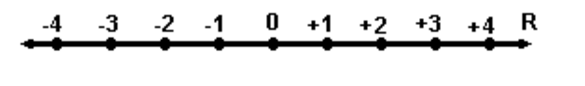
\includegraphics[width=4.39in,height=2.34in]{capitulos/logaritmos_e_funcao_logaritmica/media/image9.png}
        \end{Center}
    \end{figure}

\end{texemplo}

\begin{exercicios}
	\exitem{} Faça os gráficos das funções usando uma tabela de valores de \textit{x} e \textit{y}. (use a calculadora para encontrar os logaritmos)

    \begin{enumerate}
	    \item \textit{F(x) = log x\quad }\quad c) \textit{G(x) = log (2x)}

	    \item \textit{H(x) = 2 log x\quad }\quad d) \textit{J(x) = log (x\textsuperscript{2})}
    \end{enumerate}

    \exitem{} a) Faça o gráfico das funções \textit{y = ln x}~~~e~  \textit{y = e\textsuperscript{x}}.~ 

        b) Faça o gráfico da função \textit{y = x}.

	c) Verifique se existe simetria entre as funções \textit{y = ln x}~~~e~  \textit{y = e\textsuperscript{x}}, em relação à função identidade~~~~~ \textit{y = x}.

	\exitem{} Faça um esboço do gráfico das funções logarítmicas sem usar a tabela.
    \begin{enumerate}
	    \item \textit{F(x) = ln (2x)} \quad \quad \quad c) \textit{Y(x) = -ln (3x)}

	    \item \textit{P(x) = -log (-5x)\quad \quad \quad }d) \textit{Q(x) = 2 log (2x)} 
    \end{enumerate}

	\exitem{} Faça um esboço do gráfico e determine o domínio e a imagem das funções:

    \begin{enumerate}
	    \item \textit{F(x) = ln~(x -  2) \quad \quad }\quad c) \textit{Y(x) = -ln (3+x)}

	    \item \textit{P(x) = -ln (3- x)\quad \quad }\quad d) \textit{Q(x) = 2 log (x + 1)} 
    \end{enumerate}

	\exitem{} Utilize um aplicativo computacional para fazer o gráfico das funções. Determine o domínio e a imagem.
    \begin{enumerate}
	    \item \textit{F(x) = ln (x\textsuperscript{2}) \quad \quad }\quad c) \textit{Y(x) = ln (1-3x)}

	    \item \textit{P(x) = log \textsuperscript{2}(x)\quad \quad \quad }d) \textit{Q(x) =~ log (x\textsuperscript{2} - 1)}
    \end{enumerate}

    \exitem{} Calcule as raízes das funções:
    a) \textit{F(x) = log (2x -~ 1) \quad }\quad c) \textit{Y(x) = -log (5 - x\textsuperscript{2})}

    b) \textit{P(x) = -ln (3- 6x)\quad \quad }\quad d) \textit{Q(x) = 2 log (-x + 1)}

    \exitem{} Faça um esboço do gráfico das funções manualmente e sem fazer tabela. Interprete as informações contidas nos coeficientes.
    \begin{enumerate}
    	\item \textit{F(x) = ln x +2} \quad \quad c) \textit{Y(x) = ln x – 3 \quad }e)\textit{ R(x) = ln(-x) +1}

	    \item \textit{P(x) = -log x +3\quad }\quad d) \textit{Q(x) = 2ln x + 1 \quad }f)\textit{ T(x) = ln(-2x) -2} 
    \end{enumerate}
\end{exercicios}

\section{Aplicações de funções exponenciais e logarítmicas}

Os logaritmos, atualmente, são mais utilizados para resolução de equações exponenciais e como funções, do que para sua função original, dos tempos de Napier e Bürgi, de facilitar multiplicações e divisões de números muito pequenos ou muito grandes. Problemas de decaimento ou crescimento exponencial envolvem necessariamente o uso dos logaritmos.

\subsection{Aplicações financeiras}

Considere-se uma aplicação financeira do tipo poupança, em que um capital inicial \textit{C\textsubscript{o }=~ R$\$$  1.000,00} é depositado no mês t = 0 e é corrigido mensalmente com uma taxa de juros constante de \textit{i = 0,5 $\%$ } do capital presente. O capital a cada mês pode ser calculado da seguinte maneira:

\textit{C(1) = 1000 + 1000 $ \cdot $  (0,5/100) = 1000 $ \cdot $  (1+0,5/100) = 1000 $ \cdot $  1,005}

\textit{C(2) = 1000 $ \cdot $  1,005 $ \cdot $  1,005 = 1000 $ \cdot $  1,005\textsuperscript{2}}

\textit{C(3) = 1000 $ \cdot $  1,005\textsuperscript{2}~ $ \cdot $ ~1,005 =  1000 $ \cdot $  1,005\textsuperscript{3}}

Ou para este caso,~~ \textit{C(t) = 1000 $ \cdot $  1,005\textsuperscript{t}} ~~~ onde \textit{t} é o tempo em meses.\quad (8.1)

Com a função (8.1) pode-se calcular o capital (montante) da poupança para qualquer tempo \textit{t}. Com essa função também pode-se calcular o tempo necessário para que a poupança atinja determinado capital \textit{C}, simplesmente resolvendo (8.1) para \textit{t}:

\textit{C = 1000 $ \cdot $  1,005\textsuperscript{t}} . Dividindo por \textit{1000}, tem-se

\( \frac{C}{1000}=1,005^{t} \) .~~~ Aplicando logaritmo natural em ambos os lados da equação, tem-se

\( ln\frac{C}{1000}=ln1,005^{t}~~~~ ^{} \) . Usando a propriedade da potência, tem-se

\( ln\frac{C}{1000}=t \cdot ln1,005^{}~~~~ ^{} \) . Isolando \textit{t}, tem-se

\( t=\frac{ln\frac{C}{1000}}{ln1,005}~  \) . \qedsymbol{}

\begin{exercicios}
    \exitem{} Escreva a Eq. 8.1 na forma generalizada. Utilize~ \textit{C\textsubscript{o}} para expressar o capital inicial e~  \textit{j} ~ para a taxa de juros, sendo

    \( j=1+\frac{i}{100} \) .

	\exitem{} Calcule o capital de uma poupança sendo~ \textit{C\textsubscript{o}= R$\$$  500,00 },\textit{ i=0,45 }ao mês, depois de \textit{3 }anos.~~ 

	\exitem{} Calcule o tempo necessário de uma poupança, para que o capital atinja o valor de \textit{C =} \textit{R$\$$  20.000,00}, sendo~ \textit{C\textsubscript{o}=R$\$$  1.500,00 } e\textit{ i=0,6 }ao mês.~ 

	\exitem{} Calcule~a~taxa de juros   \textit{j}~ e a taxa de rendimento mensal \textit{~ i } de uma aplicação tipo poupança em que \textit{C\textsubscript{o}=R$\$$  500,00},~sendo~que~o~capital~inicial ficou aplicado durante 5 anos e chegou ao montante de R$\$$   2.500,00.     

	\exitem{} Um pai emprestou~ \textit{R$\$$  5.500,00} a seu filho, que demorou \textit{3} anos para pagar. Considerando a taxa de\textit{ i=0,6 }ao mês, qual é a dívida do filho?~~ 

\end{exercicios}

\subsection{Desvalorização de bens}

Alguns bens, tais como carros, apartamentos, casas, barcos e outros sofrem desvalorização com o passar do tempo. Se a cada ano o bem desvalorizasse sempre o mesmo valor teríamos uma taxa constante de desvalorização. Porém, não é o que ocorre na realidade. Na maioria dos casos essa desvalorização não é proporcional ao tempo, ou seja, a taxa de desvalorização não é constante. A Tabela 8.2.1 dá o preço de mercado de dois modelos de carro. 

Tabela 8.2.1 – Preços (em reais x 1000) de dois modelos de carro em função do tempo (em anos).

\begin{table}[H]
 			\centering
\begin{tabular}{p{0.78in}p{0.55in}p{0.49in}p{0.49in}p{0.49in}p{0.49in}p{0.49in}p{0.49in}}
\hline
%row no:1
\multicolumn{1}{|p{0.78in}}{} & 
\multicolumn{1}{|p{0.55in}}{0} & 
\multicolumn{1}{|p{0.49in}}{1} & 
\multicolumn{1}{|p{0.49in}}{2} & 
\multicolumn{1}{|p{0.49in}}{3} & 
\multicolumn{1}{|p{0.49in}}{4} & 
\multicolumn{1}{|p{0.49in}}{5} & 
\multicolumn{1}{|p{0.49in}|}{6} \\
\hhline{--------}
%row no:2
\multicolumn{1}{|p{0.78in}}{Modelo 1 (R$\$$ x1000)} & 
\multicolumn{1}{|p{0.55in}}{49} & 
\multicolumn{1}{|p{0.49in}}{43} & 
\multicolumn{1}{|p{0.49in}}{35} & 
\multicolumn{1}{|p{0.49in}}{32} & 
\multicolumn{1}{|p{0.49in}}{30} & 
\multicolumn{1}{|p{0.49in}}{28} & 
\multicolumn{1}{|p{0.49in}|}{27} \\
\hhline{--------}
%row no:3
\multicolumn{1}{|p{0.78in}}{Modelo 2 (R$\$$ x1000)} & 
\multicolumn{1}{|p{0.55in}}{30} & 
\multicolumn{1}{|p{0.49in}}{25} & 
\multicolumn{1}{|p{0.49in}}{23} & 
\multicolumn{1}{|p{0.49in}}{22} & 
\multicolumn{1}{|p{0.49in}}{20,8} & 
\multicolumn{1}{|p{0.49in}}{20} & 
\multicolumn{1}{|p{0.49in}|}{19,5} \\
\hhline{--------}

\end{tabular}
 \end{table}

Podemos associar a desvalorização de cada modelo a um número e com ele tomar a decisão de compra. Consideremos a função exponencial como o modelo matemático da desvalorização dos carros.

\textit{P(t) = P\textsubscript{o} $ \cdot $  e \textsuperscript{– kt}}{\fontsize{14pt}{16.8pt}\selectfont \textit{~~~~ \quad \quad \quad \quad \quad \quad \quad }(8.2.1)}

Onde \textit{P} é o preço (em R$\$$ x1000), \textit{P\textsubscript{o}~ }é o preço do carro novo, \textit{t} é o tempo (anos) e \textit{k} é a constante característica da depreciação, de cada modelo de carro. A depreciação será maior, quanto maior for o valor de \textit{k}. 

Para calcular o valor de \textit{k}, precisamos resolver a Eq. (8.2.1) para \textit{k}. Dividindo esta equação por \textit{P\textsubscript{o}}, temos:

\( \frac{P \left( t \right) }{P_{0}}=e^{-kt} \) .~ 

Aplicando logaritmo natural em ambos os lados da equação e usando a propriedade P3 dos logaritmos, temos:

\( ln \left( \frac{P \left( t \right) }{P_{0}} \right) =-kt  \) . dividindo por (\textit{– t}) (para \textit{t $ \neq $  0}), temos:

\( k=-\frac{1}{t}ln \left( \frac{P \left( t \right) }{P_{0}} \right)  \) \quad \quad \quad \quad \quad \quad \quad (8.2.2)

Se aplicamos a Eq.(8.2.2) para cada ano, obteremos, para esse exemplo, seis valores de \textit{k}, cuja média chamaremos de \textit{k} médio (\textit{k\textsubscript{m}}). Para os dados da Tab. 8.2.1 obtivemos os seguinte valores:

\quad Modelo 1: \textit{k\textsubscript{m} = 0,12913}

\quad Modelo 2: \textit{k\textsubscript{m} = 0,1105}.

Portanto, o Modelo 2 tem depreciação menor que o Modelo 1.

Levando \textit{k\textsubscript{m}} na Eq.(8.2.1) no lugar de \textit{k}, obtemos uma função que descreve a desvalorização do modelo em função do tempo (Eq. 7.2.3).

\( P \left( t \right) =P_{0}e^{-k_{m}t} \) \textit{.\quad \quad \quad \quad \quad \quad \quad }(8.2.3)

\begin{figure}[H]
	\begin{Center}
		\includegraphics[width=4.0in,height=2.32in]{capitulos/logaritmos_e_funcao_logaritmica/media/image10.png}
	\end{Center}
\end{figure}

A Figura 8.2.1 apresenta os dados da Tab. 8.2.1 (pontos) e as curvas de depreciação (curvas ajustadas) obtidas com a Eq. 8.2.3 e os respectivos valores de \textit{k\textsubscript{m}}~ para os modelos 1 e 2.\qedsymbol{}

\subsection{Linearização de gráficos de funções exponenciais}

Em algumas aplicações de funções exponenciais do tipo 

\textit{y = f(x) = Ae\textsuperscript{kx}} , 

podemos~escrever  \textit{f(x)} com uma reta, aplicando logaritmo natural nos dois lados da equação e usando a propriedade do produto, temos:

\textit{ln y = ln A~~+~  ln e\textsuperscript{kx}}. Usando a propriedade P3 dos logaritmos, temos:

\textit{ln y = ln A~ + kx~.~  }Fazendo\textit{ Y = ln y~ }e\textit{~~b =  ln a, }temos:

\textit{Y = b + kx.\quad \quad \quad \quad \quad \quad \quad \quad \quad }(8.3.1)

A Eq. (8.31) é uma equação de reta, onde \textit{b} é o coeficiente linear e \textit{k} o angular. Com esta equação, o cálculo de \textit{k} ou de \textit{x} fica elementar:

\( k=\frac{1}{x} \left( Y-b \right)  \) ~~~~~~ e~~~  \( x=\frac{1}{k} \left( Y-b \right)  \) .

\subsection{Crescimento ou decrescimento populacional}

{\fontsize{14pt}{16.8pt}\selectfont \textbf{8.4.1 – Crescimento de bactérias }}

A quantidade de bactérias que se reproduzem por mitose (cada ser se divide em dois seres idênticos), considerando que não haja morte de indivíduos, pode ser modelada da seguinte maneira: 

Geração~ zero :~1 bactéria  

1ª geração :~2 bactéria  ; \textit{P = 2\textsuperscript{1}}

2ª geração : 4 bactéria ; \textit{P = 2\textsuperscript{2}}

3ª geração : 8 bactéria ; \textit{P = 2\textsuperscript{3}}

4ª geração : 16 bactéria;~ \textit{P = 2\textsuperscript{4}}

5ª geração : 32 bactéria;~ \textit{P = 2\textsuperscript{5}}

A função\textit{~~ P(n) = 2\textsuperscript{n}~~ \quad \quad \quad \quad \quad \quad \quad \quad }(8.4.1)

onde \textit{P} é o número de bactérias e \textit{n }é a geração, permite calcular a população para qualquer tempo, desde que se saiba o tempo \textit{t} necessário para a reprodução de uma geração. Por exemplo, se \textit{n = 5}~ e \textit{t = 2 h}, em \textit{10} horas a população é \textit{32} bactérias. 

Se precisamos saber em quanto tempo a população atingirá 5000 indivíduos, aplicamos logaritmo de base \textit{2} na Eq. 8.4.1 e temos :

\( log_{2}P=log_{2}2^{n} \) . Utilizando a propriedade P3 dos logaritmos, temos:

\( n=log_{2}P \) . Usando \textit{P = 5000}, temos:

\( n=log_{2}5000 \)  . Escrevendo este logaritmo na base e, temos:

\( n=\frac{ln5000}{ln2}=12,28 \)  gerações. Ou, aproximadamente \textit{12} gerações, o que significa \textit{24 h}.

{\fontsize{14pt}{16.8pt}\selectfont \textbf{8.4.2 – Decaimento bacteriano}}

As bactérias que vivem no organismo humano, quando colocadas na água ou no solo, não sobrevivem por muito tempo. Assim, a população de bactérias presentes nos esgotos tende a diminuir. O fenômeno é conhecido como $``$decaimento bacteriano$"$  e é modelado pela função 

\textit{P(t) = P\textsubscript{o} $ \cdot $  e \textsuperscript{– kt}}{\fontsize{14pt}{16.8pt}\selectfont \textit{~~~~ \quad \quad \quad \quad \quad \quad \quad }(8.4.2)}

Onde \textit{P} é a população (número de indivíduos), \textit{P\textsubscript{o}~ }é a população inicial, \textit{t} é o tempo (horas) e \textit{k} é a constante ou taxa característica do decaimento, a qual depende de vários fatores, dentre eles o tipo de bactéria, a temperatura e a acidez do ambiente. O decaimento será maior, quanto maior for o valor de \textit{k}. 

Geralmente, o interesse de um pesquisador é determinar o tempo necessário para que metade da população seja exterminada. Esse tempo é conhecido como \textit{meia vida}. Na meia vida a população é \textit{P = P\textsubscript{o}/2}. Substituindo esse valor de P na Eq. 8.4.2, temos:

\textit{ P\textsubscript{o}/2= P\textsubscript{o} $ \cdot $  e \textsuperscript{– kt}}{\fontsize{14pt}{16.8pt}\selectfont \textit{~ ~ . }Cancelando\textit{ P\textsubscript{o} .}}

\( \frac{1}{2}=e^{-kt} \) {\fontsize{14pt}{16.8pt}\selectfont \textit{. }Aplicando logaritmo natural nos dois lados da equação e isolando \textit{t}, temos\textit{ }}

{\fontsize{14pt}{16.8pt}\selectfont \textit{ }}

\( t=-\frac{1}{k}~~ ln  \left( \frac{ 1}{2} \right)  \) {\fontsize{14pt}{16.8pt}\selectfont ~ que é a meia vida.}

\subsection{Concentração de medicamentos no organismo humano}

Quando um medicamento é ingerido a corrente sanguínea o distribui por todo o organismo. Consideremos que a concentração (massa, em gramas, por unidade de volume de sangue) é a mesma em cada parte do corpo. A eliminação do medicamento ocorre na medida que o sangue vai passando pelos rins. Portanto, uma função concentração (C(t)) é decrescente, e tem um valor máximo inicial C\textsubscript{o}. Supondo que a variação da concentração seja uma função da massa medicamento presente no organismo, podemos propor um modelo exponencial, com a seguinte função:

\begin{FlushRight}
 \( C \left( t \right) =C_{o}e^{at} \) \quad \quad \quad \quad \quad \quad (8.5.1)
\end{FlushRight}

Onde \textit{C} é a concentração do medicamento (\textit{g}), \textit{C\textsubscript{o}} é a dose inicial, \textit{t} é o tempo e \textit{a} uma constante real, sendo \textit{a < 0}.

O tempo de meia-vida, ou simplesmente a meia-vida~ ($ \tau$ )~é~o tempo necessário para que metade da quantidade inicial   \textit{C\textsubscript{o}} seja eliminada. É comum usar a ideia de meia-vida para investigar a variação da concentração de medicamentos no sangue. Assim, fazendo \textit{C}($ \tau$ ) \textit{= C\textsubscript{o}/2} e substituindo em (8.5.1), temos:

\begin{FlushRight}
 \( \frac{C_{o}}{2}=C_{o}e^{a \tau} \) \quad \quad \quad \quad \quad \quad (8.5.2)
\end{FlushRight}

Cancelando \textit{C\textsubscript{o}} , aplicando logaritmo natural em ambos os membros de (8.5.2) e resolvendo para $ \tau$ , temos uma expressão para o tempo de meia-vida:

\begin{FlushRight}
 \(  \tau=-\frac{1}{a}ln2 \) \quad \quad \quad \quad \quad \quad (8.5.3)
\end{FlushRight}

Se a meia-vida do medicamento é conhecida, podemos resolver a Eq. (8.5.3) para \textit{a}. 

\begin{FlushRight}
 \( a=-\frac{1}{ \tau}ln2 \) \quad \quad \quad \quad \quad \quad (8.5.4)
\end{FlushRight}

{\fontsize{14pt}{16.8pt}\selectfont \textbf{8.5.1 – Concentração do medicamento: dose única}}

Consideremos um medicamento cuja meia-vida é \textit{$ \tau$  = 4 h} e a dose \textit{C\textsubscript{o} = 800 mg}. Com a Eq.(4) podemos calcular \textit{a}, obtendo \textit{a = -0,17329}. Substituindo estes dados na Eq. (8.5.1), temos uma função que dá valores da concentração para cada instante de tempo, da dose inicial.

\begin{FlushRight}
 \( C \left( t \right) =800e^{-0,17329 t} \) \quad \quad \quad \quad (8.5.5)
\end{FlushRight}

A Fig. 1 apresenta os valores da concentração obtidos com a função da Eq.(5), onde pode-se verificar que o tempo para a eliminação da metade da dose inicial (meia-vida) é \textit{4 h} e que em torno de \textit{40h} a concentração é mínima, para estes dados. É importante observar que a posição da curva depende da meia-vida do medicamento, que é, em resumo, um ponto da curva onde \textit{C = C\textsubscript{o}/2} e que caracteriza o comportamento do medicamento no organismo. 

\begin{figure}[H]
	\begin{Center}
		\includegraphics[width=5.01in,height=3.01in]{capitulos/logaritmos_e_funcao_logaritmica/media/image11.jpeg}
	\end{Center}
\end{figure}

{\fontsize{14pt}{16.8pt}\selectfont \textbf{8.5.2 – Concentração do medicamento: doses múltiplas}}

Consideremos que um paciente tenha ingerido o medicamento de 8 em 8h (intervalo de tempo de ingestão) e que cada dose seja eliminada com a mesma meia-vida. Para calcular a concentração total em função do tempo, devemos calcular a concentração de cada dose independentemente, utilizando a Eq.(8.5.1). Somando as concentrações em tempo de ingestão, obtemos a concentração de todas as doses em função do tempo. A Tab. 1 apresenta este método e foi obtida com os mesmos dados do item \textbf{8.5.1} (dose única). 

Observando as somas (Total) em função do tempo, percebemos elas tendem a um valor específico, que é o limite da concentração do medicamento no organismo. Esse efeito pode ser observado claramente na Fig.8.5.2.

\textbf{Tabela 8.5.1} – Concentração do medicamento para múltiplas doses

\begin{table}[H]
 			\centering
\begin{tabular}{p{0.47in}p{0.47in}p{0.47in}p{0.47in}p{0.47in}p{0.52in}p{0.52in}p{0.52in}p{0.52in}}
\hline
%row no:1
\multicolumn{1}{|p{0.47in}}{}{\begin{tabular}{p{0.47in}}Doses\\\end{tabular}} & 
\multicolumn{8}{|p{5.18in}|}{\Centering Tempo (h)} \\
\hhline{~--------}
%row no:2
\multicolumn{1}{|p{0.47in}}{} & 
\multicolumn{1}{|p{0.47in}}{0} & 
\multicolumn{1}{|p{0.47in}}{8} & 
\multicolumn{1}{|p{0.47in}}{16} & 
\multicolumn{1}{|p{0.47in}}{24} & 
\multicolumn{1}{|p{0.52in}}{32} & 
\multicolumn{1}{|p{0.52in}}{40} & 
\multicolumn{1}{|p{0.52in}}{48} & 
\multicolumn{1}{|p{0.52in}|}{56} \\
\hhline{---------}
%row no:3
\multicolumn{1}{|p{0.47in}}{1} & 
\multicolumn{1}{|p{0.47in}}{400} & 
\multicolumn{1}{|p{0.47in}}{100} & 
\multicolumn{1}{|p{0.47in}}{25} & 
\multicolumn{1}{|p{0.47in}}{6,25} & 
\multicolumn{1}{|p{0.52in}}{1,5625} & 
\multicolumn{1}{|p{0.52in}}{0,390625} & 
\multicolumn{1}{|p{0.52in}}{0,097656} & 
\multicolumn{1}{|p{0.52in}|}{0,024414} \\
\hhline{---------}
%row no:4
\multicolumn{1}{|p{0.47in}}{2} & 
\multicolumn{1}{|p{0.47in}}{} & 
\multicolumn{1}{|p{0.47in}}{400} & 
\multicolumn{1}{|p{0.47in}}{100} & 
\multicolumn{1}{|p{0.47in}}{25} & 
\multicolumn{1}{|p{0.52in}}{6,25} & 
\multicolumn{1}{|p{0.52in}}{1,5625} & 
\multicolumn{1}{|p{0.52in}}{0,390625} & 
\multicolumn{1}{|p{0.52in}|}{0,097656} \\
\hhline{---------}
%row no:5
\multicolumn{1}{|p{0.47in}}{3} & 
\multicolumn{1}{|p{0.47in}}{} & 
\multicolumn{1}{|p{0.47in}}{} & 
\multicolumn{1}{|p{0.47in}}{400} & 
\multicolumn{1}{|p{0.47in}}{100} & 
\multicolumn{1}{|p{0.52in}}{25} & 
\multicolumn{1}{|p{0.52in}}{6,25} & 
\multicolumn{1}{|p{0.52in}}{1,5625} & 
\multicolumn{1}{|p{0.52in}|}{0,390625} \\
\hhline{---------}
%row no:6
\multicolumn{1}{|p{0.47in}}{4} & 
\multicolumn{1}{|p{0.47in}}{} & 
\multicolumn{1}{|p{0.47in}}{} & 
\multicolumn{1}{|p{0.47in}}{} & 
\multicolumn{1}{|p{0.47in}}{400} & 
\multicolumn{1}{|p{0.52in}}{100} & 
\multicolumn{1}{|p{0.52in}}{25} & 
\multicolumn{1}{|p{0.52in}}{6,25} & 
\multicolumn{1}{|p{0.52in}|}{1,5625} \\
\hhline{---------}
%row no:7
\multicolumn{1}{|p{0.47in}}{5} & 
\multicolumn{1}{|p{0.47in}}{} & 
\multicolumn{1}{|p{0.47in}}{} & 
\multicolumn{1}{|p{0.47in}}{} & 
\multicolumn{1}{|p{0.47in}}{} & 
\multicolumn{1}{|p{0.52in}}{400} & 
\multicolumn{1}{|p{0.52in}}{100} & 
\multicolumn{1}{|p{0.52in}}{25} & 
\multicolumn{1}{|p{0.52in}|}{6,25} \\
\hhline{---------}
%row no:8
\multicolumn{1}{|p{0.47in}}{6} & 
\multicolumn{1}{|p{0.47in}}{} & 
\multicolumn{1}{|p{0.47in}}{} & 
\multicolumn{1}{|p{0.47in}}{} & 
\multicolumn{1}{|p{0.47in}}{} & 
\multicolumn{1}{|p{0.52in}}{} & 
\multicolumn{1}{|p{0.52in}}{400} & 
\multicolumn{1}{|p{0.52in}}{100} & 
\multicolumn{1}{|p{0.52in}|}{25} \\
\hhline{---------}
%row no:9
\multicolumn{1}{|p{0.47in}}{7} & 
\multicolumn{1}{|p{0.47in}}{} & 
\multicolumn{1}{|p{0.47in}}{} & 
\multicolumn{1}{|p{0.47in}}{} & 
\multicolumn{1}{|p{0.47in}}{} & 
\multicolumn{1}{|p{0.52in}}{} & 
\multicolumn{1}{|p{0.52in}}{} & 
\multicolumn{1}{|p{0.52in}}{400} & 
\multicolumn{1}{|p{0.52in}|}{100} \\
\hhline{---------}
%row no:10
\multicolumn{1}{|p{0.47in}}{8} & 
\multicolumn{1}{|p{0.47in}}{} & 
\multicolumn{1}{|p{0.47in}}{} & 
\multicolumn{1}{|p{0.47in}}{} & 
\multicolumn{1}{|p{0.47in}}{} & 
\multicolumn{1}{|p{0.52in}}{} & 
\multicolumn{1}{|p{0.52in}}{} & 
\multicolumn{1}{|p{0.52in}}{} & 
\multicolumn{1}{|p{0.52in}|}{400} \\
\hhline{---------}
%row no:11
\multicolumn{1}{|p{0.47in}}{TOTAL} & 
\multicolumn{1}{|p{0.47in}}{400} & 
\multicolumn{1}{|p{0.47in}}{500} & 
\multicolumn{1}{|p{0.47in}}{525} & 
\multicolumn{1}{|p{0.47in}}{531,25} & 
\multicolumn{1}{|p{0.52in}}{532,8125} & 
\multicolumn{1}{|p{0.52in}}{533,2031} & 
\multicolumn{1}{|p{0.52in}}{533,3008} & 
\multicolumn{1}{|p{0.52in}|}{533,3252} \\
\hhline{---------}
\end{tabular}
\end{table}

\begin{figure}[H]
	\begin{Center}
		\includegraphics[width=5.01in,height=3.01in]{capitulos/logaritmos_e_funcao_logaritmica/media/image12.jpeg}
	\end{Center}
\end{figure}

\begin{exercicios}

    \exitem{} Utilize a Eq. 8.2.3 para calcular o valor do carro Modelo 1 depois de 10 anos.

	\exitem{} Pesquise dados de preços médios de carro de seu interesse na Tabela Fipe, para ao menos, 5 anos. Repita os procedimentos do Exemplo 8.2 e calcule \textit{k\textsubscript{m}}. Faça um gráfico de Preço por tempo, para visualizar a curva de depreciação do carro.

	\exitem{} Um apartamento custava R$\$$  500.000,00 em 2000, R$\$$  450.000,00 em 2010 e R$\$$  400.000,00 em 2014. Determine o coeficiente de desvalorização~ \textit{k\textsubscript{m}\textsuperscript{ }}.

	\exitem{} Utilize a ideia de linearização das funções exponenciais para calcular \textit{k\textsubscript{m}} na equação de desvalorização de bens (Eq. 8.2.1).

	\exitem{} Utilize a ideia de linearização das funções exponenciais para calcular~ \textit{t }na equação de desvalorização de bens (Eq. 8.2.1).

	\exitem{} Se uma população de bactérias decresce, em um determinado período, de acordo com a função \textit{P(t) = 100e\textsuperscript{-0,5t}}, onde \textit{P} é o número de indivíduos e t é o tempo em minutos:

	\exitem{} Aplique logaritmo na expressão da função, para escrevê-la na forma da Eq. 8.3.1. Determine os coeficientes angular e linear.

	\exitem{} Calcule o tempo em que a população será 1/3 da população inicial (100 indivíduos).

	\exitem{} Faça o gráfico das funções \textit{P(t)} e da função linearizada obtida no ítem~(a).  



	\exitem{} Uma população de bactérias se reproduz em função do tempo de acordo com a função  \textit{P(t) = 2\textsuperscript{t} :}

	\exitem{} Calcule o número de bactérias depois de \textit{100s}. 

	\exitem{} Em quanto tempo a população será de \textit{500} indivíduos.

	\exitem{} Calcule a taxa \textit{k} de decaimento (Eq. 8.4.2), sendo que em \textit{80} s a população se reduziu à metade da população inicial.

	\exitem{} Em um tempo \textit{t = 0 h} a população de bactérias era de \textit{1000000} de indivíduos. Passadas \textit{6 h} a população se reduziu à metade da população inicial. Qual será a população quando \textit{t = 9 h} ?

	\exitem{} Sabendo que a meia vida de uma população é de \textit{3 h}:

	\exitem{} Qual é o valor da taxa de decaimento \textit{k} ?

	\exitem{} Em quanto tempo a população se reduzirá a \textit{P\textsubscript{o}/4} ?


    \exitem{} Utilizando as Eqs. (8.5.1) a (8.5.3) e uma tabela eletrônica, calcule as concentrações de um medicamento ingerido em dose única para um período de \textit{48 h}, com \textit{C\textsubscript{o} = 500mg/cm\textsuperscript{3}}~~ com os seguintes tempos de meia-vida: (apresente os resultados em um mesmo gráfico)

    a)~ \textit{$ \tau$ ~ = 5 h} \quad \quad b)~ \textit{$ \tau$ ~ = 8 h~ \quad ~~~ }c)~ \textit{$ \tau$ ~ = 10 h~ \quad }d)~ \textit{$ \tau$ ~ = 12 h~ }

    \exitem{} Desenvolva uma tabela eletrônica semelhante à Tab. 8.5.1, de maneira que a meia-vida, a dose inicial e o tempo de ingestão sejam manipuláveis pelo usuário. Calcule a concentração de medicamentos para os seguintes dados:

    a) Dados \textit{$ \tau$ ~ = 4 h~ }e \textit{C\textsubscript{o} = 800mg/cm\textsuperscript{3 }}, determine o intervalo de ingestão para que a concentração máxima seja próxima de \textit{1000} \textit{mg/cm\textsuperscript{3}}~.~~~  

    b) Dados \textit{$ \tau$ ~ = 4 h~ }e \textit{C\textsubscript{o} = 800mg/cm\textsuperscript{3}}, determine o intervalo de ingestão para a concentração máxima fique próxima de \textit{915 mg/cm\textsuperscript{3}} .

\end{exercicios}

\section{RESPOSTAS DOS EXERCÍCIOS PROPOSTOS}

\begin{respostas}{2}

    \ansitem{} a) 3\quad \quad b) 6\quad \quad c) 3/2\quad \quad d) -3 \quad \quad e) 2\quad \quad f) -5/2

    \ansitem{} a) 5\quad \quad b) -4\quad \quad c) -2\quad \quad d) 3\quad \quad e) 5\quad \quad f) $\frac{1}{4}$

~~ \quad g) -5\quad \quad h) -2/3\quad \quad i) -1/2

    \ansitem{} a) 81\quad \quad b) 2\quad \quad c)  \( \sqrt[125]{5} \) \quad d)  \( 2+2\sqrt[]{2} \) \quad e) -2\quad \quad f) 2

    \ansitem{} Não faz sentido calcular um logaritmo de base 1, pois ao aplicar a definição teremos 1\textsuperscript{n}= x, e independente de \textit{n} será encontrado x = 1, devido a uma propriedade das potências onde 1\textsuperscript{n }= 1.

    \ansitem{} Não faz sentido calcular um logaritmo com base negativa pois em determinadas equações não será possível encontrar um número que satisfaça a identidade.

    \ansitem{}Não faz sentido calcular o logaritmo de um número negativo, pois nem sempre será possível encontrar uma solução que pertença aos números reais.

    \ansitem{} 0 < x < 1

    \ansitem{} a) x > 2\quad b) x > $\frac{1}{4}$\quad c) x > $\frac{1}{2}$ e x $ \neq $  1\quad d) x > 4

\end{respostas}

\begin{respostas}{3}

    \ansitem{} a) -3\quad \quad b) -4\quad \quad c) 11\quad \quad d) $\frac{1}{4}$

    \ansitem{} a) 16\quad \quad b) 40\quad \quad c) 3\quad \quad d) 2\quad \quad e) 3\quad f) 625/2

    \ansitem{} Pela propriedade P7 temos que  \(  \left( -1 \right) log_{a}y=log_{a}y^{-1} \). Usando P4,~temos \( a^{log_{a} \left( y \right) ^{-1}}=y^{-1}=\frac{1}{y} \) .

    \ansitem{} a) ln 3\quad = 1,0986...\quad b) 2/5\quad \quad c)  \( \sqrt[]{ln600} \)  = 2,5292....\quad d)~  \( \sqrt[]{1+ln\frac{2}{3}} \) 

    \ansitem{}  \( \frac{25}{9} \)

    \ansitem{} a) V = 1,411 x 10\textsuperscript{18~~ }~~~~~ b) V = 1,411 x 10\textsuperscript{18}
\end{respostas}

\begin{respostas}{4}

    \ansitem{} a) 1\quad \quad b) 5 \quad \quad c) 3\quad \quad d) 10\quad \quad e) -5\quad \quad f) -3\quad 

    \ansitem{} a) 0,3010...\quad b) 1,9459...\quad c) 1,3010...\quad d) 1,8450...\quad e) 2,8903...\quad f) 4

\quad g) 1\quad \quad h) 0

\ansitem{} a) 1,5849...\quad b) 0,4306...\quad c) 1,4306...\quad d) 1,6094...

\ansitem{} a) 1,5849...\quad b) 0,4306...\quad c) 1,4306...\quad d) 0,6989...

\ansitem{} a)  \( \frac{log_{}2}{log_{}e} \) \quad b)  \( \frac{log_{}20}{log_{}e} \) \quad c)  \( \frac{log_{}18}{log_{}e} \) \quad d)  \( \frac{log_{}e}{log_{}e}=1 \) {\fontsize{14pt}{16.8pt}\selectfont  }

\ansitem{} a)  \( \frac{ln25}{ln10} \) \quad \quad b)  \( \frac{ln7}{ln10} \) \quad \quad c)  \( \frac{-ln5}{ln10} \) \quad \quad d)  \( \frac{ln3-ln4}{ln10} \) 

\ansitem{} - 0,1249... = (0,4771...) – (0,6020) = - 0,1249...

\end{respostas}

\begin{respostas}{5}

	\ansitem{} a) 2\quad \quad b) 1\quad \quad c) 1\quad \quad d) S=$ \{ $  \( \sqrt[]{10},100 \) $ \} $ 

    \ansitem{} a)  \( \frac{log10}{log2} \) \quad b)  \( \sqrt[]{\frac{ln100}{2}} \) \quad c)  \( -\frac{2}{3} \) \quad ~~~~ d)  \( \frac{log2}{4} \) \quad e) S=$ \{ $ 1,3$ \} $ \quad f) 4 \textbf{+} log 2

    \ansitem{} a) -2\quad \quad b) 2\quad \quad c) S=$ \{ $ -2,0$ \} $ \quad d)  \( \frac{3}{8} \) 

    \ansitem{} É possível resolver usando a definição de logaritmo.

    \ansitem{} a) 2\quad \quad b) S=$ \{ $ -1,3$ \} $ \quad c)  \( \frac{1}{2} \) \quad 

    \ansitem{} É possível resolver usando a definição de logaritmo.

    \ansitem{} a) 100\quad ~~~ b) 10\textsuperscript{5\quad }c)  \( \sqrt[]{\frac{3}{100}} \) \quad d)  \( \frac{3}{10^{5}} \) \quad \quad e)  \( \frac{23}{3} \) \quad \quad f) S=$ \{ $ 1,9$ \} $ 

    \ansitem{} a) 8\quad \quad b) 10/ln4\quad c)  \( \sqrt[3]{3} \) \quad \quad d) ln$^2$4

    \ansitem{} Aproximadamente 381 meses.

    \ansitem{} \( t= \frac{log\frac{C}{C0}}{log(x) \left( 1+\frac{i}{100} \right) } \)

    \ansitem{} \( t= -\frac{1}{k}ln \left( \frac{1}{2} \right)  \) 

    \ansitem{} a) (usar \textit{u = log x});~ \textit{x\textsubscript{1} = 100}~~e  \textit{x\textsubscript{2} = 0,1}~~~~~~~~~ b) 9\quad \quad c)  \( \sqrt[]{2} \) \quad \quad d)  \( \sqrt[]{10} \) 
\end{respostas}

\begin{respostas}{6}
	\ansitem{} \quad a) f(g(x)) = 9x$^2$-6x+1 ; g(f(x)) = 3x$^2$-1\quad b) f(g(x)) = x ; g(f(x)) = x

\quad c) f(g(x)) = x ; g(f(x)) = x\quad \quad \quad d) f(g(x)) = x ; g(f(x)) = x

    \ansitem{} a,b,d são funções inversas; c não é inversa

    \ansitem{} a) 

    \begin{figure}[H]
	    \begin{Center}
		    \includegraphics[width=2.91in,height=2.23in]{capitulos/logaritmos_e_funcao_logaritmica/media/image13.png}
	    \end{Center}
    \end{figure}

b)

    \begin{figure}[H]
	    \begin{Center}
		    \includegraphics[width=2.77in,height=2.31in]{capitulos/logaritmos_e_funcao_logaritmica/media/image14.png}
        \end{Center}    
    \end{figure}

    \ansitem{}
    
    \begin{figure}[H]
	    \begin{Center}
		    \includegraphics[width=2.9in,height=2.26in]{capitulos/logaritmos_e_funcao_logaritmica/media/image15.png}
	    \end{Center}
    \end{figure}

    \begin{figure}[H]
	    \begin{Center}
		    \includegraphics[width=2.91in,height=2.24in]{capitulos/logaritmos_e_funcao_logaritmica/media/image16.png}
	    \end{Center}
    \end{figure}

	\ansitem{}

	\ansitem{} a)  \( \sqrt[]{x-3} \) \quad b) x\textsuperscript{4}-2\quad \quad c) ln (x/5) – 2\quad d) 10

    \ansitem{} a) 

    \begin{figure}[H]
	    \begin{Center}
	    	\includegraphics[width=2.95in,height=2.68in]{capitulos/logaritmos_e_funcao_logaritmica/media/image17.png}
	    \end{Center}
    \end{figure}

    b)

    \begin{figure}[H]
	    \begin{Center}
		    \includegraphics[width=2.76in,height=2.57in]{capitulos/logaritmos_e_funcao_logaritmica/media/image18.png}
	    \end{Center}
    \end{figure}

    \ansitem{} \colorbox{red}{c)}
    \ansitem{} \colorbox{red}{d)}

    \ansitem{} A composição da direta de todas as funções sobre suas inversas resultam em x.

    \ansitem{} a) Crescente para x > 0

    \ansitem{} b) Crescente para x > -2

    \ansitem{} c) Decrescente para x < 0

    \ansitem{} d) Crescente para x < 1

\end{respostas}

\begin{respostas}{7}
	\ansitem{} a) 

    \begin{figure}[H]
	    \begin{Center}
    		\includegraphics[width=2.58in,height=1.83in]{capitulos/logaritmos_e_funcao_logaritmica/media/image19.jpeg}
    	\end{Center}
    \end{figure}

b)

    \begin{figure}[H]
	    \begin{Center}
    		\includegraphics[width=2.55in,height=1.98in]{capitulos/logaritmos_e_funcao_logaritmica/media/image20.jpeg}
	    \end{Center}
    \end{figure}

c)

    \begin{figure}[H]
	    \begin{Center}
		    \includegraphics[width=2.56in,height=1.81in]{capitulos/logaritmos_e_funcao_logaritmica/media/image21.jpeg}
	    \end{Center}
    \end{figure}

d)

\begin{figure}[H]
	\begin{Center}
		\includegraphics[width=2.56in,height=2.0in]{capitulos/logaritmos_e_funcao_logaritmica/media/image22.jpeg}
	\end{Center}
\end{figure}

	\ansitem{} a)

    \begin{figure}[H]
	    \begin{Center}
	    	\includegraphics[width=2.54in,height=1.93in]{capitulos/logaritmos_e_funcao_logaritmica/media/image23.JPG}
	    \end{Center}
    \end{figure}

    \begin{figure}[H]
	    \begin{Center}
    		\includegraphics[width=2.55in,height=1.78in]{capitulos/logaritmos_e_funcao_logaritmica/media/image24.JPG}
    	\end{Center}
    \end{figure}

    b)

    \begin{figure}[H]
	    \begin{Center}
		    \includegraphics[width=2.55in,height=1.94in]{capitulos/logaritmos_e_funcao_logaritmica/media/image25.JPG}
        \end{Center}    
    \end{figure}

    c) Em relação a reta y = x é possível notar que a função \textit{ln x} é simétrica a \textit{e\textsuperscript{x}}. 

	\ansitem a)

\begin{figure}[H]
	\begin{Center}
		\includegraphics[width=2.56in,height=1.81in]{capitulos/logaritmos_e_funcao_logaritmica/media/image26.JPG}
	\end{Center}
\end{figure}

b)

\begin{figure}[H]
	\begin{Center}
		\includegraphics[width=2.56in,height=1.78in]{capitulos/logaritmos_e_funcao_logaritmica/media/image27.JPG}
	\end{Center}
\end{figure}

c)

\begin{figure}[H]
	\begin{Center}
		\includegraphics[width=2.55in,height=1.84in]{capitulos/logaritmos_e_funcao_logaritmica/media/image28.JPG}
	\end{Center}
\end{figure}

d)

\begin{figure}[H]
	\begin{Center}
		\includegraphics[width=2.56in,height=1.64in]{capitulos/logaritmos_e_funcao_logaritmica/media/image29.JPG}
	\end{Center}
\end{figure}

	\ansitem{} a)

\begin{figure}[H]
	\begin{Center}
		\includegraphics[width=2.58in,height=1.6in]{capitulos/logaritmos_e_funcao_logaritmica/media/image30.JPG}
	\end{Center}
\end{figure}

b)

\begin{figure}[H]
	\begin{Center}
		\includegraphics[width=2.58in,height=1.55in]{capitulos/logaritmos_e_funcao_logaritmica/media/image31.JPG}
	\end{Center}
\end{figure}

c)

\begin{figure}[H]
	\begin{Center}
		\includegraphics[width=2.56in,height=1.62in]{capitulos/logaritmos_e_funcao_logaritmica/media/image32.JPG}
	\end{Center}
\end{figure}

d)

\begin{figure}[H]
	\begin{Center}
		\includegraphics[width=2.55in,height=1.61in]{capitulos/logaritmos_e_funcao_logaritmica/media/image33.JPG}
	\end{Center}
\end{figure}

\ansitem{} a)

D = $ \{ $  x $ \in $ R $ \} $ 

Im = $ \{ $  y $ \in $ R$ \} $ 

\begin{figure}[H]
	\begin{Center}
		\includegraphics[width=2.57in,height=1.6in]{capitulos/logaritmos_e_funcao_logaritmica/media/image34.JPG}
	\end{Center}
\end{figure}

b)

D = $ \{ $  x  \(  \in R \)  / x > 0$ \} $ 

Im = $ \{ $  y  \(  \in R \)  / y $ \geq $  0$ \} $ 

\begin{figure}[H]
	\begin{Center}
		\includegraphics[width=2.57in,height=1.69in]{capitulos/logaritmos_e_funcao_logaritmica/media/image35.JPG}
	\end{Center}
\end{figure}

c)

D = $ \{ $ x $ \in $ R / x < 1/3$ \} $ 

Im = $ \{ $  y $ \in $ R $ \} $ 

\begin{figure}[H]
	\begin{Center}
		\includegraphics[width=2.55in,height=1.6in]{capitulos/logaritmos_e_funcao_logaritmica/media/image36.JPG}
	\end{Center}
\end{figure}

d)

D = $ \{ $  x $ \in $ R / -1 > x > 1$ \} $ 

Im = $ \{ $  y $ \in $ R$ \} $ 

\begin{figure}[H]
	\begin{Center}
		\includegraphics[width=2.55in,height=1.66in]{capitulos/logaritmos_e_funcao_logaritmica/media/image37.JPG}
	\end{Center}
\end{figure}


\ansitem{}  a) 1\quad \quad b) 1/3\quad \quad c) 0\quad \quad d) 0

\end{respostas}

\begin{respostas}{8}

    \ansitem{} C(t)=C\textsubscript{0}.j\textsuperscript{t}

    \ansitem{} 587,71 reais

    \ansitem{} 36,08 meses

    \ansitem{} 2,7 $\%$  ao mês 

    \ansitem{} 6 821, 65 reais

    \ansitem{} 13,47 (xR$\$$ 1000)

    \ansitem{} k\textsubscript{m}=0,013234...

    \ansitem{} k\textsubscript{m}=  \( -\frac{1}{t} . ln(x) \left( \frac{P}{P \left( 0 \right) } \right)  \)  

    \ansitem{} t=  \( -\frac{1}{x} .ln \left( \frac{P}{P \left( 0 \right) } \right)  \) 

\end{respostas}